\documentclass[a4paper, 11pt]{tufte-handout}
% \documentclass[a4paper, 11pt]{article}
\usepackage[margin=0.8in]{geometry}
\usepackage{framed}
\usepackage{graphicx}
\usepackage{xcolor}
\usepackage{blindtext}
\usepackage{xcolor}
\usepackage{mdframed}
\usepackage{indentfirst}
\usepackage{graphicx}
\usepackage{subcaption}
\usepackage{hyperref}
%\usepackage{txfonts}
\usepackage{amsmath}
\usepackage{titling}
\usepackage{titlesec}
\usepackage[brazil]{babel}
\definecolor{LightGray}{gray}{0.97}
\usepackage{minted}
\usepackage{xcolor}

\setminted[fortran]{  framesep=2mm,
  baselinestretch=1.2,
  bgcolor=LightGray,
  fontsize=\footnotesize,
  linenos}

\titleformat{\section}{\normalfont\Large\bfseries}{\thesection}{1em}{}[\titlerule] 
\titleformat{\subsection}{\normalfont\large\bfseries}{\thesubsection}{1em}{} 
% \renewcommand\thesubsection{\Alph{subsection}}
\graphicspath{ {./graficos/} }
\hypersetup{
  pdfauthor={Jefter Santiago},
  pdftitle={Projeto 4 - Modelos de crescimento},
  pdfcreator={Jefter Santiago}, 
  pdflang={Portuguese},
  colorlinks=true,    % Color links instead of boxes
  linkcolor=blue,     % Color of internal links
  citecolor=green,    % Color of citation links
  urlcolor=blue,      % Color of URLs
}
\begin{document}
\noindent
\large\textbf{Autor:} Jefter Santiago \hfill \textbf{Projeto 4 - {\color{blue}\emph{Modelos de Crescimento}}}   \\
\#USP: 12559016 \\
\normalsize Curso: Física Estatística Computacional \hfill 2024.1 \\
Prof. F. C. Alcaraz \hfill Data de entrega: 04/05/20.3 \\
\noindent\rule{7in}{2.8pt}


\section{Autômatos celulares deterministícos (ACD)}

Começamos o estudo de modelo de crescimendo partindo de um modelo determinístico. Os
\emph{ACDs} consistem em uma regra que transforma uma configuração de uma grade (no nosso
caso unidimensional) em outra, ou seja, se tivermos a configuração \( \mathcal{C}_{t}\) uma regra \( \mathcal{F}\)
nos fornece \( \mathcal{C}_{t + 1} \).

Para uma cadeia de \( L \) sítios consideramos dois possíveis estados, \( 1 \) ou \( 0 \), e o
estado futuro de um sítio dependerá dos dois sítios adjacentes\footnote{Assumindo condições
periódicas de contorno.}. Dessa forma, para qualquer sítio \( i \), temos a tupla de \( 3 \)
componentes que definem seu estado em \( t + 1 \). Logo, um conjunto \( \{ b_{i-1}, b_i, b_{i+i} \}
\) tem \( 2^3 \) possíveis estados, como os estados são binários, no total teremos \( 2^{8} = 256 \)
estados possiveis para um sítio.


Sabendo disso podemos gerar realizar simulações de autômatos celulares partindo de regrais quaisquer
e utilizando a representação binário do número para calcular o próximo estado de um sítio.



Nosso interesse é simular o automatos com 3 configurações iniciais: todos os sítios \( 0 \) , todos
\( 1 \) e uma configuração aleatória. Foram feitas as simulações para as regras $232$\footnote{``Regra
  da maioria''.}, \( 254 \)\footnote{``Regra da epidêmia''.} e a regra  $51$.\footnote{``Regra do contra''.}


Segue o código implementado para os \emph{ACDs}:


\begin{marginfigure}
  \centering
  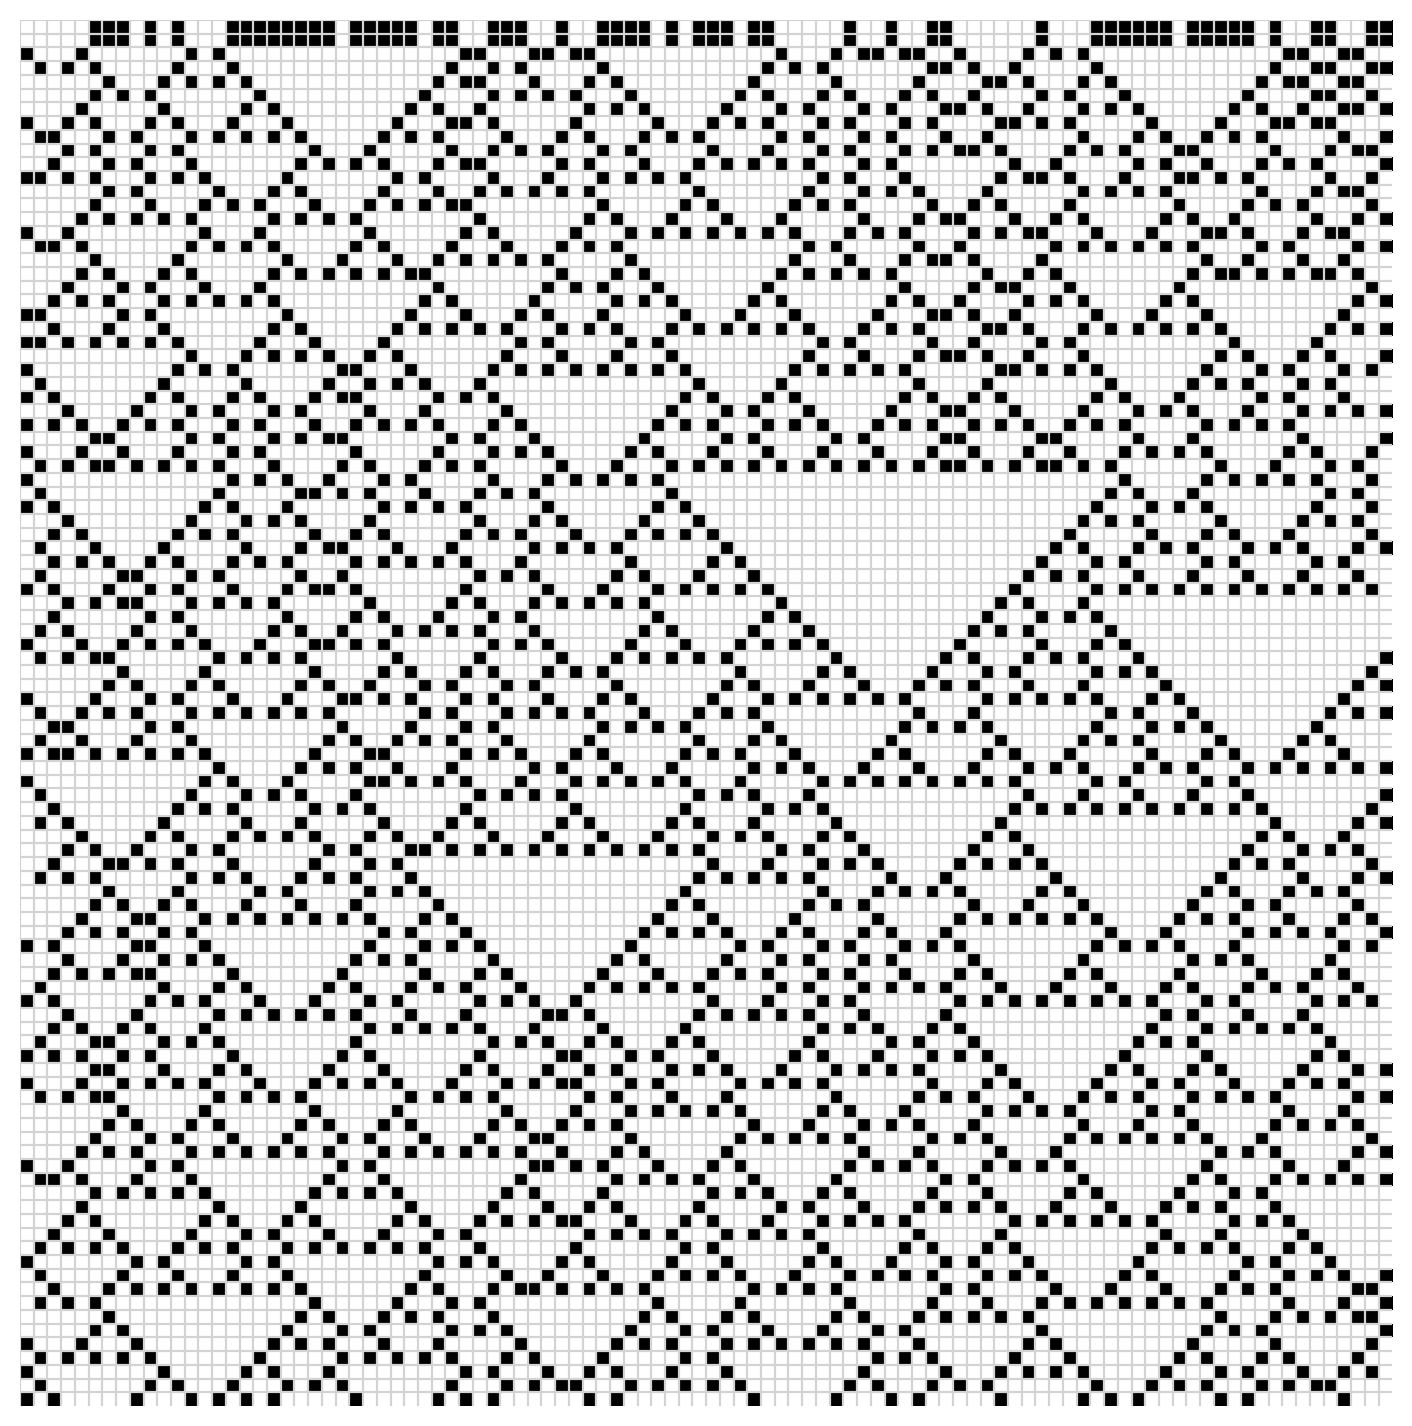
\includegraphics[width=0.75\textwidth]{tarefa-1/rule-18-0.png}
  \caption{Regra 18.}
  \label{fig:fig_rule18}
\end{marginfigure}

\begin{marginfigure}
  \centering
  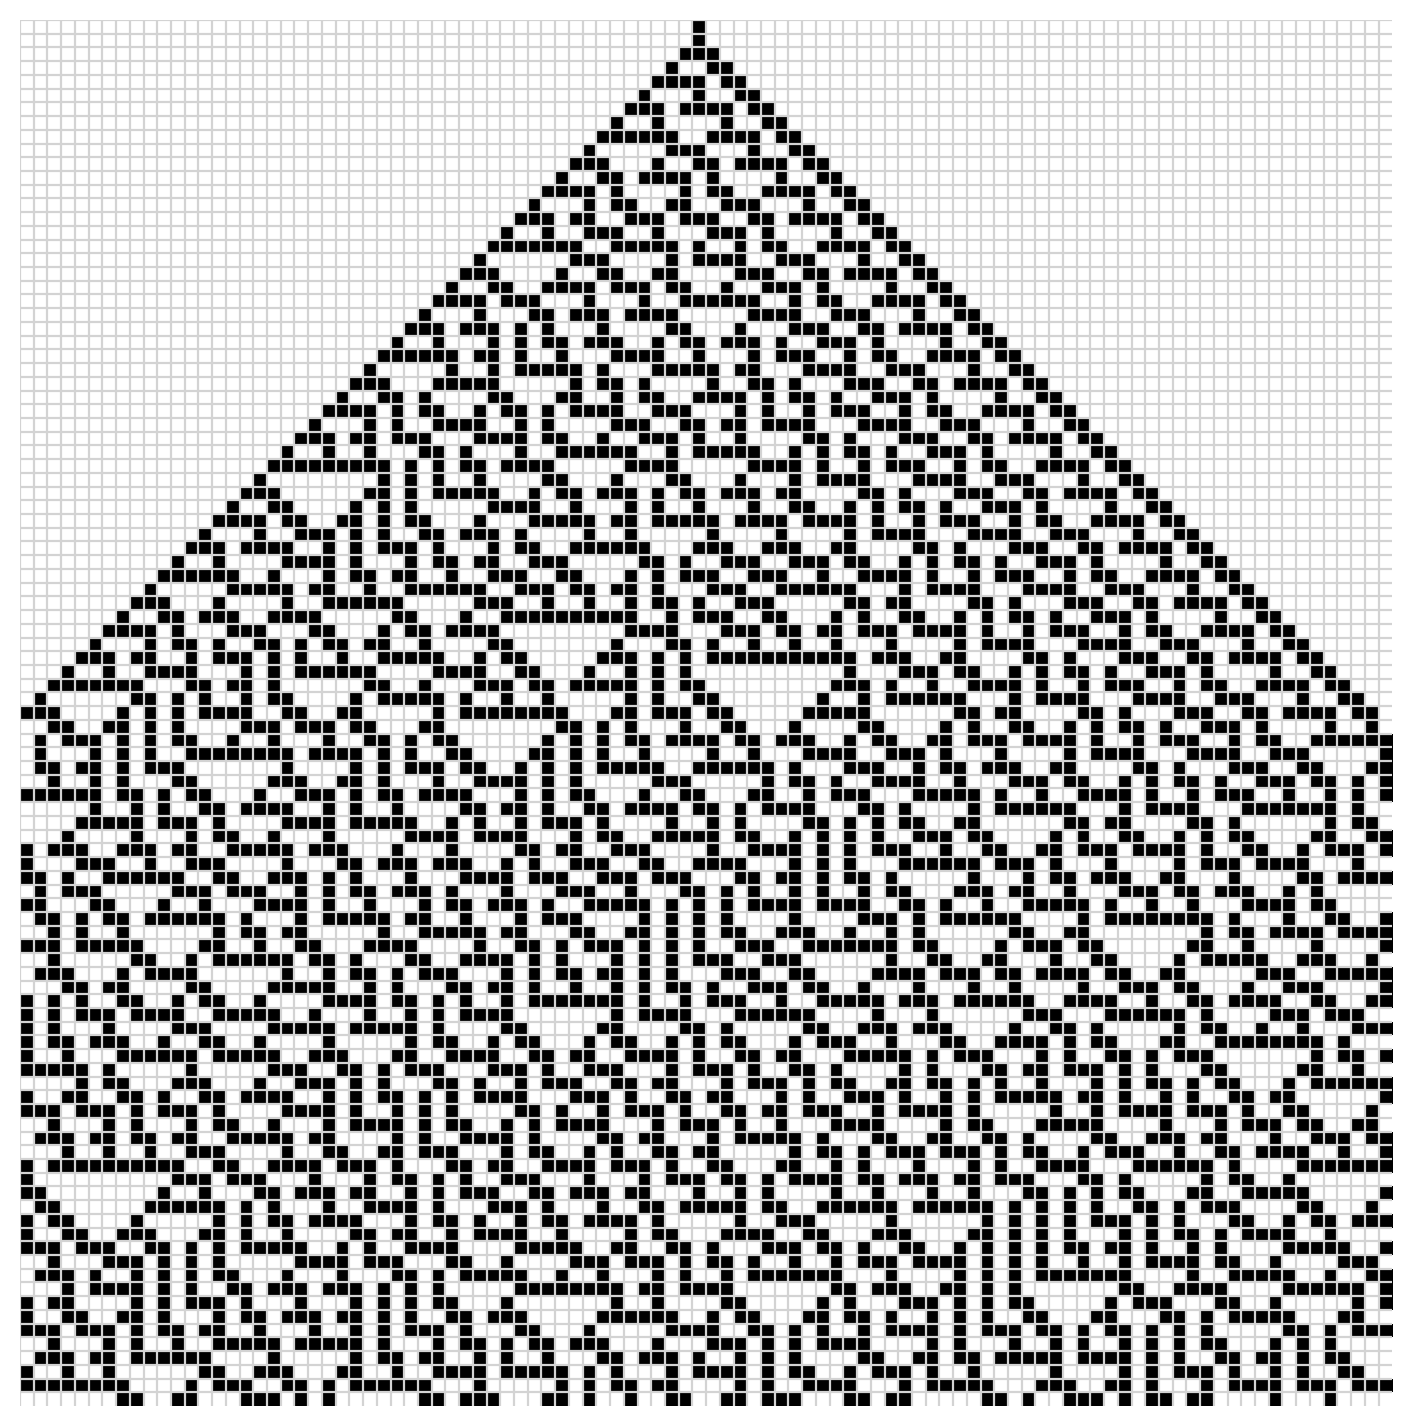
\includegraphics[width=0.75\textwidth]{tarefa-1/rule-86-0.png}
  \caption{Regra 86}
  \label{fig:fig_rule86}

\end{marginfigure}
\begin{minted}{fortran}
!     Gera estado inicial da cadeia.
!     Se config = 0 => C_0¹ = {0, ..., 0} 
!     Se config = 1 => C_0² = {1, ..., 1}
!     Se config qualquer outro valor => C_0³ = {b_1,..., b_L}
!     com b_i aleatorio.
      subroutine set_initial_state(C, config, L)
      implicit integer (c-c)
      dimension C(500)

      if(config == 0) then
         C(:) = 0
      else if (config == 1) then
         C(:) = 1
      else
         p = rand(iseed)
         do i = 1, L
            p = rand() * 2
!           k in [0, 1]
            k = int((p+1) / 2)
!            print *, k
            C(i) = k
         end do
      end if
      end subroutine

!     Popula o vetor rules de 8 posições
!     com valores 0 ou 1
!     a partir de um número inteiro
!     entre 0, 255
      subroutine rule_set(rules, N)
      implicit integer(r-r)
      dimension rules(8)
      M = N
!      print *, "N = ", N
!      print *, "M = ", M
      do i = 1, 8
         x = real(M)
         rules(i) = mod(M, 2)
         M = int(x/2.0)
      end do

!      do i = 1, 8
!         print *, rules(i)
!      end do

      end subroutine


      subroutine propagate(C, rules, L)
      implicit integer(c-c, r-r)
      dimension rules(8)
      ! C_{t}
      dimension C(500)
      ! C_{t+1}
      dimension C_tmp(500)

      do i = 2, L-1
         C_tmp(i) = rules(4*C(i-1)+2*C(i)+C(i+1)+1)
      end do

      C_tmp(1) = rules(4*C(L)+2*C(1)+C(2)+1)
      C_tmp(L) = rules(4*C(L-1)+2*C(L)+C(1)+1)

      C = C_tmp

      end subroutine

      
      ! Max size of chain; L = 500
      subroutine DCA(rule_number, N_iter, L, init_state, f_name)
      implicit integer(f-f, c-c, r-r)
      dimension rules(8)
      dimension C(500)

!      print *, "rule_number = ", rule_number
      call set_initial_state(C, init_state, L)

      write(f_name, *) (C(j), j = 1, L)

      call rule_set(rules, rule_number)

      do i = 1, N_iter
         write(f_name, *) (C(j), j = 1, L)
         call propagate(C, rules, L)
      end do
      end subroutine DCA

      ! Max size of chain; L = 500
      subroutine DCA_position(rule_number, N_iter, L, pos, f_name)
      implicit integer(f-f, c-c, r-r, p-p)
      dimension rules(8)
      dimension C(500)

!      print *, "rule_number = ", rule_number
      call set_initial_state(C, 0, L)
      C(pos) = 1

      write(f_name, *) (C(j), j = 1, L)

      call rule_set(rules, rule_number)

      do i = 1, N_iter
         write(f_name, *) (C(j), j = 1, L)
         call propagate(C, rules, L)
      end do
      end subroutine DCA_position
\end{minted}

\begin{marginfigure}
  \centering
  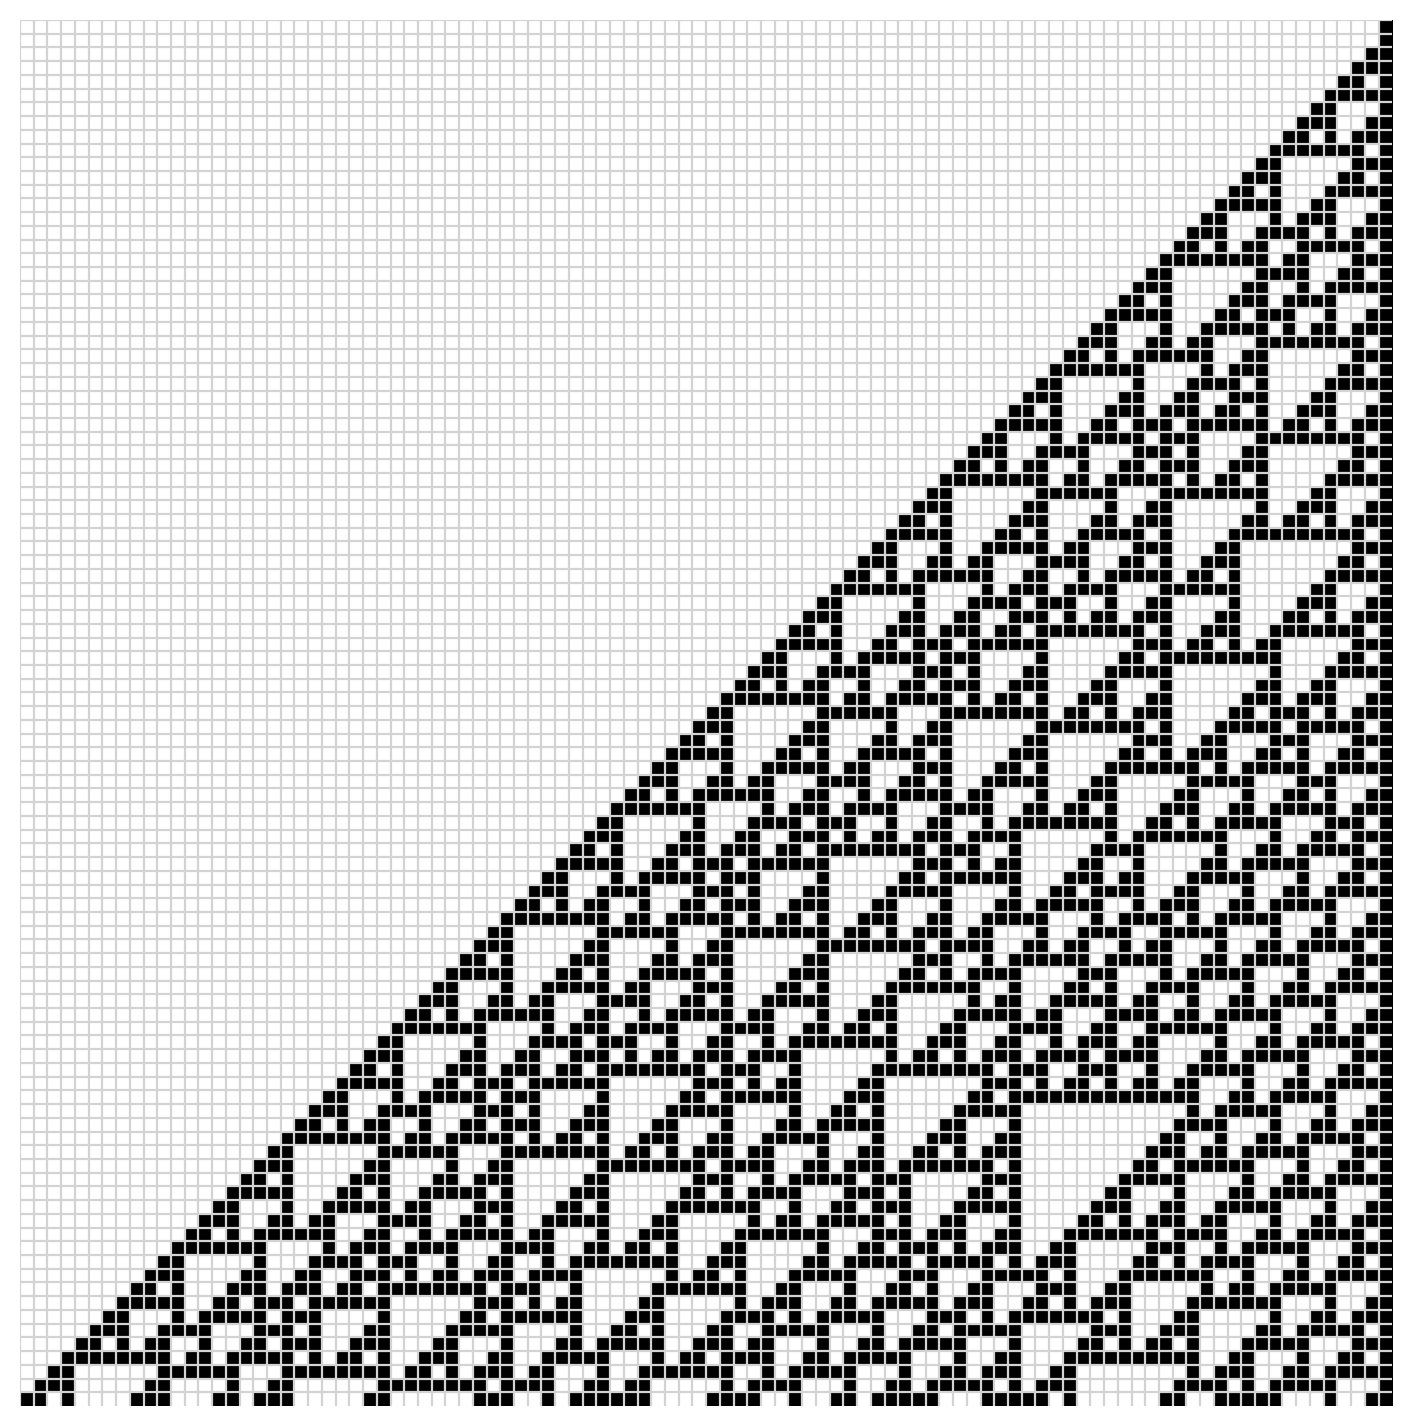
\includegraphics[width=0.75\textwidth]{tarefa-1/rule-110-0.png}
  \caption{Regra 110.}
  \label{fig:fig_rule110}
\end{marginfigure}



Essas rotinas estão no arquivo \verb|tarefa-1/cellular-automaton.f| e são utilizadas
no programa principal \verb|tarefa-1/tarefa-1.f|:

\begin{minted}{fortran}
      implicit integer (c-c, r-r)
      ! C_{t}
      L = 100
      K = 100
      print *, "Forneca regra R [0, 255]"

      read(*, *) R
      
      open(unit = 1, file="rule-#-0.dat")
      open(unit = 2, file="rule-#-1.dat")
      open(unit = 3, file="rule-#-2.dat")

      call DCA(R, K, L, 0, 1)
      call DCA(R, K, L, 1, 2)
      call DCA(R, K, L, 2, 3)

      close(1)
      close(2)
      close(3)
      end
\end{minted}


Segue abaixo as imagens da evolução dos automatos celulares executados pelo \verb|tarefa-1/tarefa-1.f|:

\begin{figure}[h]
  \centering
  
\includegraphics[width=0.3\textwidth]{tarefa-1/rule-51-0.png}
  
\includegraphics[width=0.3\textwidth]{tarefa-1/rule-51-1.png}
  
\includegraphics[width=0.3\textwidth]{tarefa-1/rule-51-2.png}
  \caption{Regra $51$.}
\end{figure}
\begin{figure}[h]
  \centering
  
\includegraphics[width=0.3\textwidth]{tarefa-1/rule-232-0.png}
  
\includegraphics[width=0.3\textwidth]{tarefa-1/rule-232-1.png}
  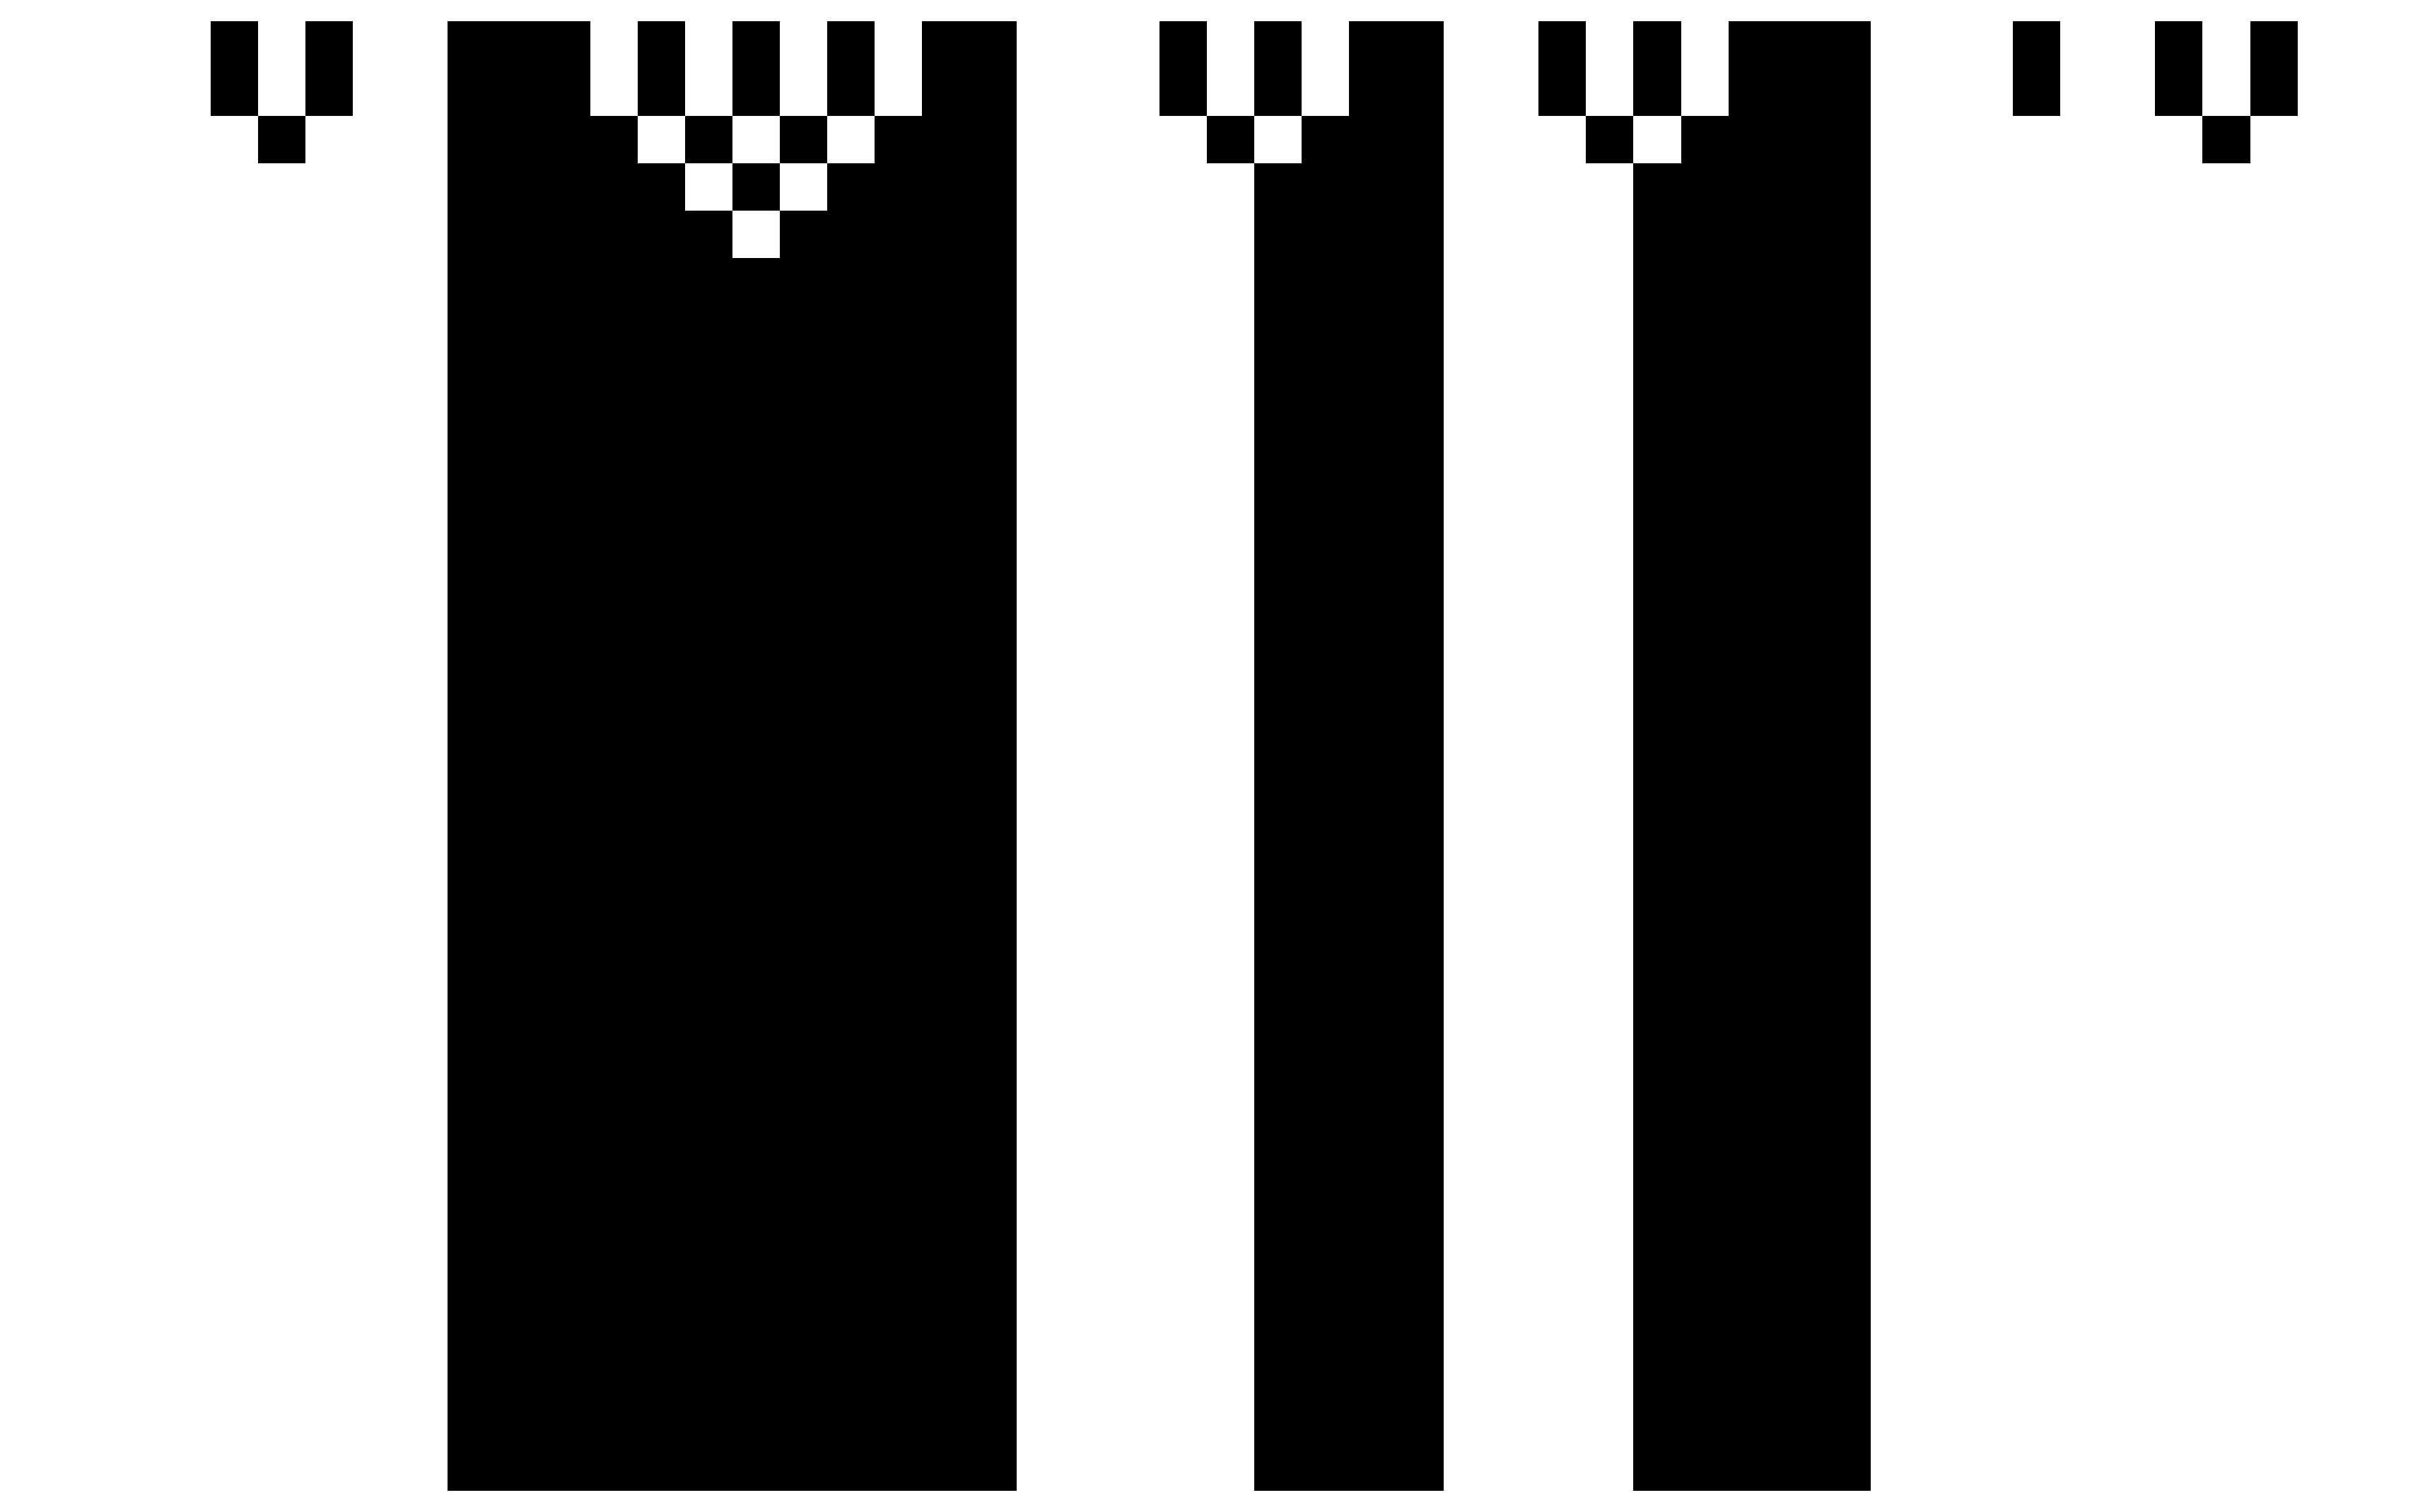
\includegraphics[width=0.3\textwidth]{tarefa-1/rule-232-2.png}
  \caption{Regra $232$.}
\end{figure}
\begin{figure}[h!]
  \centering
  
\includegraphics[width=0.3\textwidth]{tarefa-1/rule-254-0.png}
  
\includegraphics[width=0.3\textwidth]{tarefa-1/rule-254-1.png}
  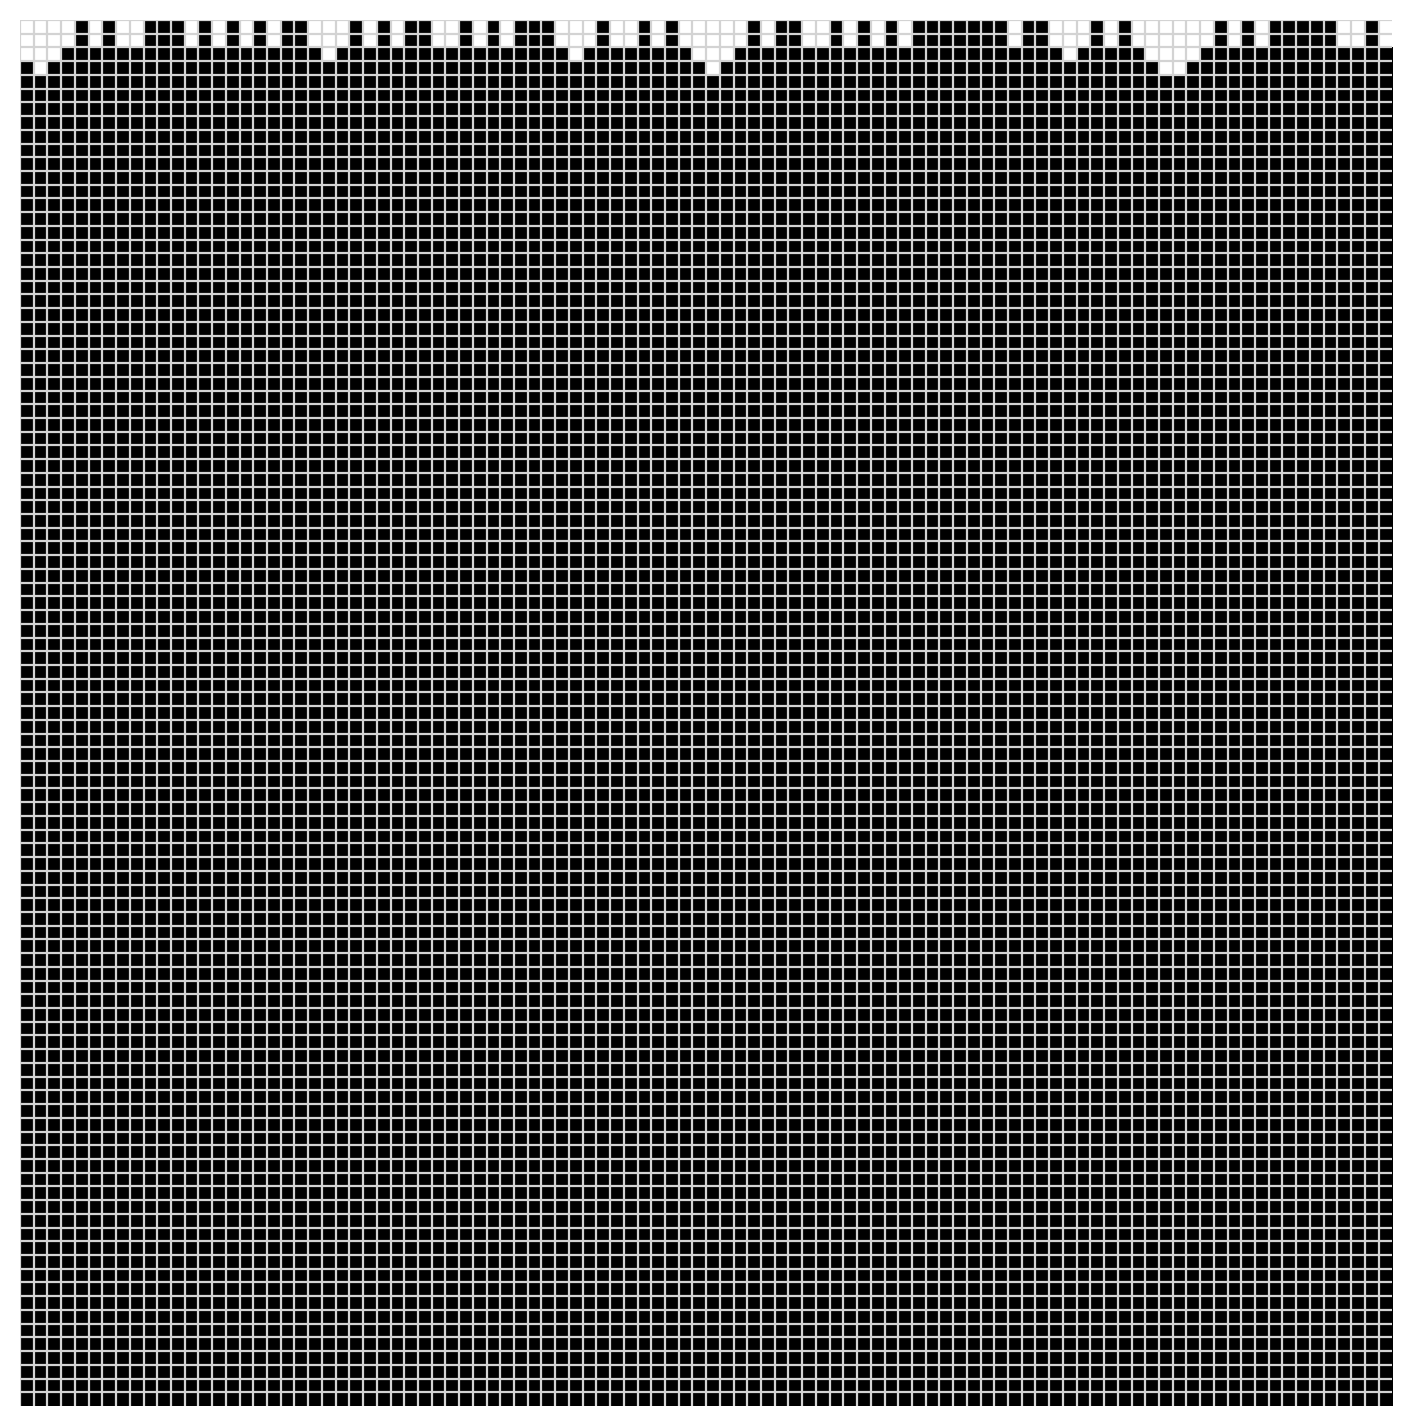
\includegraphics[width=0.3\textwidth]{tarefa-1/rule-254-2.png}
  \caption{Regra $254$.}
\end{figure}


Além desses padrões, também feito uma variação do programa principal e um script
externo em \emph{bash} que executa o programa para todas as regras possíveis de \( 0 \) à \( 255 \).
Esse script é o \verb|tarefa-1/all-rules.sh| e deve ser tornado executável para executar o programa
\verb|tarefa-1/all-rules.f|. As configurações são salvas no diretório
\verb|saidas/tarefa-1/all-rules/| e além disso os gráficos ficam em uma pasta de mesmo nome no
diretório \verb|graficos/|. Algumas das outras regras estão nas figuras (\ref{fig:fig_rule18})
,(\ref{fig:fig_rule86}),(\ref{fig:fig_rule110}).




\clearpage
\section{DLA 2D}
O principal modelo de crescimento estudado foi do \emph{Diffusion limited agregation}, que é um
modelo de crescimento aleatório. Nesse modelo deixamos utilizamos de random walks para observar um
padrão de crescimento para um agloramerado de partículas. Além implementar a simulação e observar
graficamente o resultado final do aglomerado, também foi realizado o cálculo da dimensão fractal
associada à esse tipo de crescimento.

Na simulação centramos nossa semente inicial sempre na origem do sistema de coordenadas e
então adotamos um raio \( R_i \) no qual outras partículas devem inicializar seu movimento
aleatório. Partículas que excedem uma distância maior que um fator \( \beta = 1.5 \) do tamanho do raio
inicial são descartas\footnote{E a simulação delas iniciada novamente.}. Partículas que atingem o
agregado passam a compô-lo. Além disso, sempre que adicionamos novas partículas ao corpo é feita uma
checagem sobre o tamanho do raio atual, se necessário este é atualizado.

À cada adição de novas partículas ao agregado, também somamos o número de partículas total para o
raio atual, dessa forma no arquivo de saida do programa temos dados para observar o crescimento
do número de partículas em função do raio $N(r)$ e determinar qual a dimensão fractal da simulação.


Segue abaixo o código para implementação do \emph{DLA-2D}. \footnote{Assim como anteriormente, o código é um
conjunto das subrotinas e o programa principal é \verb|tarefa-2/tarefa-2.f|.}

\begin{minted}{fortran}
!     Dinâmica DLA em 2D
!     Para cada partícula:
!     - Gera posicao inicial aleatoria.
!     - Aplica dinâmica de random walk.
!     - Ao agregar novas celulas armazena a posição e raio atual à um
!     arquivo de dados.
!     Parâmetros:
!     Np -> numero de particulas
      subroutine DLA_2D(Np, iseed)
      implicit integer (x-x, y-y)
      parameter(N = 500)
      dimension lattice(-N:N, -N:N)

!     semente inicial
      lattice(0, 0) = 1
     
      rnd = rand(iseed)
      
      R_in = 5.0
      R_f = 1.5 * R_in

      open(1, file="saida-dla.dat")
      open(2, file="saida-contagem.dat")

      nparts = 0

      do i = 1, Np

         x = 0
         y = 0

         print *, "Particle #", i

         call generate_random_particle(R_in, x, y) 

         s = 0
         touched = 0

         do while(touched == 0) 

            call random_step(x, y) 

            d = sqrt(real(x**2 + y ** 2))
            
!     Captura celula ao redor da posição atual se houver
            do k = -1, 1
               do j = -1, 1
!                Checagem de borda
                  if(abs(x) < N .and. abs(y) < N)then
                     s = s + lattice(x+k, y+j)
                  end if
               end do
            end do
!     Adiciona nova celula, atualiza raio
            if (d >= R_f) then
               touched = 1
            else if(s >= 1) then
               touched = 1
!     Adiciona mais uma particula à conta do raio.
               lattice(x, y) = 1
!     Salva o cluster
               nparts = nparts + 1
               write(1, *) x, y, R_in
               write(2, *) R_in, nparts

               if(d > R_in) then
                  R_in = d + 5
                  R_f = 1.5 * R_in
               end if
            end if
         end do
      end do
      close(2)
      end subroutine DLA_2D
!     Gera uma partícula em uma posicao aleatoria
!     dado um raio inicial R_in
      subroutine generate_random_particle(R_in, x, y)
      implicit integer (c-c, x-x, y-y)
      parameter(pi = acos(-1e0))

      rnd_val = rand()

      theta = 2 * pi * rnd_val

      x = int(R_in * cos(theta))
      y = int(R_in * sin(theta))

      end subroutine generate_random_particle

!     Dinâmica das particulas.
!     Executa random-walk até que: atinge uma celula ocupada
!     Parametros:
!     posicao x, y
      subroutine random_step(x,y)
      implicit integer(x-x,y-y)

      x = x + floor(rand()*3) - 1
      y = y + floor(rand()*3) - 1

      end subroutine random_step
\end{minted}


O programa principal é simplesmente:

\begin{minted}{fortran}
  !   DLA (2D)
      read(*, *) iseed
      call DLA_2D(50000, iseed)
      end 
\end{minted}
Como na tarefa anterior, também foi criado um arquivo \verb|.sh| para executar o \verb|tarefa-2.exe|
para alguns diferentes \emph{seeds} e mover os outputs para o diretório de saídas.

\clearpage


A figura (\ref{fig:dla_2d}) é o resultado da simulação para algumas seeds de número aleatório
diferentes. O gráfico de calor foi feito a partir da magnitude da distância normalizada para cada um
dos plots, sendo os pontos mais escuros mais próximos da semente inicial da simulação e mais claros
são mais distântes.

\begin{figure*}[h!]
  \centering
  \includegraphics[width=0.8\textwidth]{tarefa-2/DLA_2D-graf.png}
  \caption{DLA 2D: Configuração final dos agregados para semenetes 169, 255 e 954, respectivamente.}
  \label{fig:dla_2d}
\end{figure*}


Analisando puramente a contagem do número de pontos em um dado raio podemos obter o seguinte
gráfico(\ref{fig:n_r_fractal}): 

\begin{figure}[h!]
  \centering
  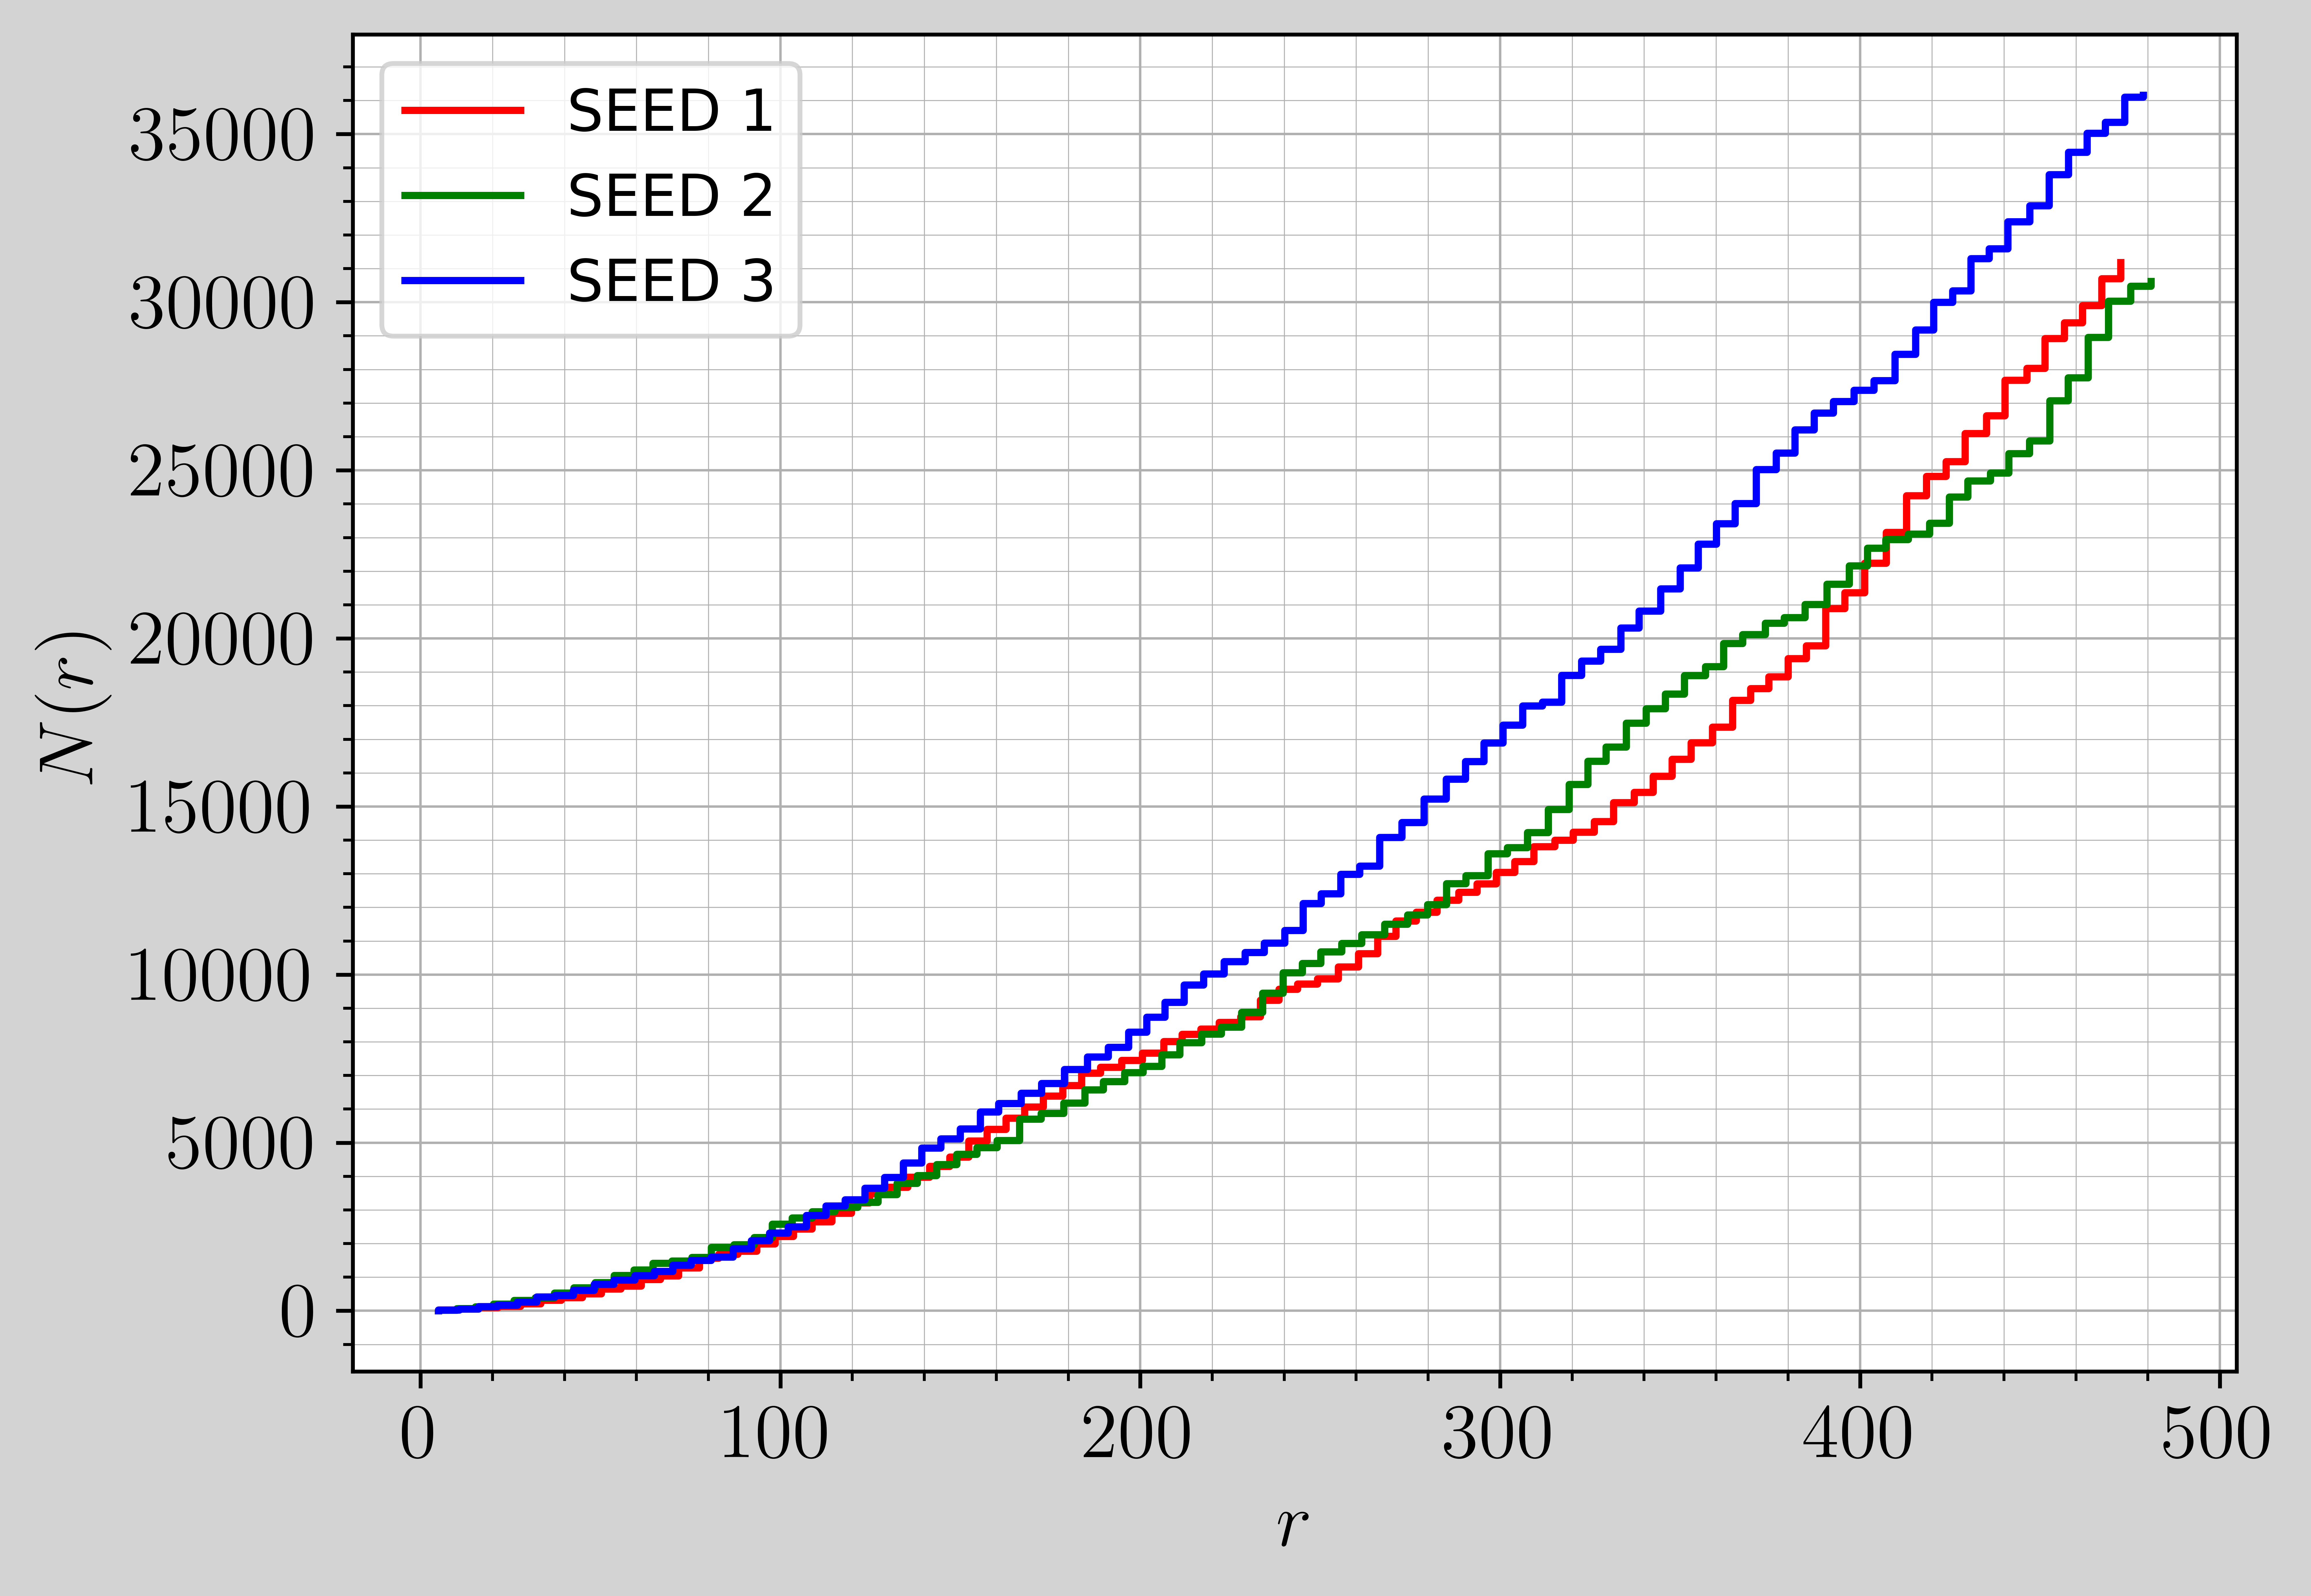
\includegraphics[width=0.65\textwidth]{tarefa-2/tarefa2-graf-pontos-raio.png}
  \caption{Número de pontos em relação ao raio.}
  \label{fig:n_r_fractal}
\end{figure}


Colocando em \emph{log}$\times$\emph{log} e realizando regressão linear obtemos a dimensão fractal
\( d_f \) para cada uma das simulações.

\begin{figure*}
  \centering
  \includegraphics[width=0.65\textwidth]{tarefa-2/tarefa2-graf-regressao-linear-dimensao-fractal.png}
  \caption{Gráfico da dimensão fractal em \emph{log}$\times$\emph{log} e regressão linear.}
  \label{fig:dim_fractal}
\end{figure*}

Isto, é, para a \emph{SEED 1} temos \( d_f \approx 1,69 \), \emph{SEED 2} \( d_f \approx 1,64 \)  e
\emph{SEED 3} \( d_f \approx 1,76  \). Esses valores estão dentro do esperado para o \emph{DLA} em duas
dimensões. 


\clearpage
\section{DLA 3D}


O modelo \emph{DLA} em 3D não oferece nenhuma grande dificuldade de implementação, já que podemos
aproveitar boa parte do código implementado no anterior. É esperado que  a dimensão fractal seja
maior que a do modelo anterior com  \( 2 < d_f < 3\).

\begin{marginfigure}
  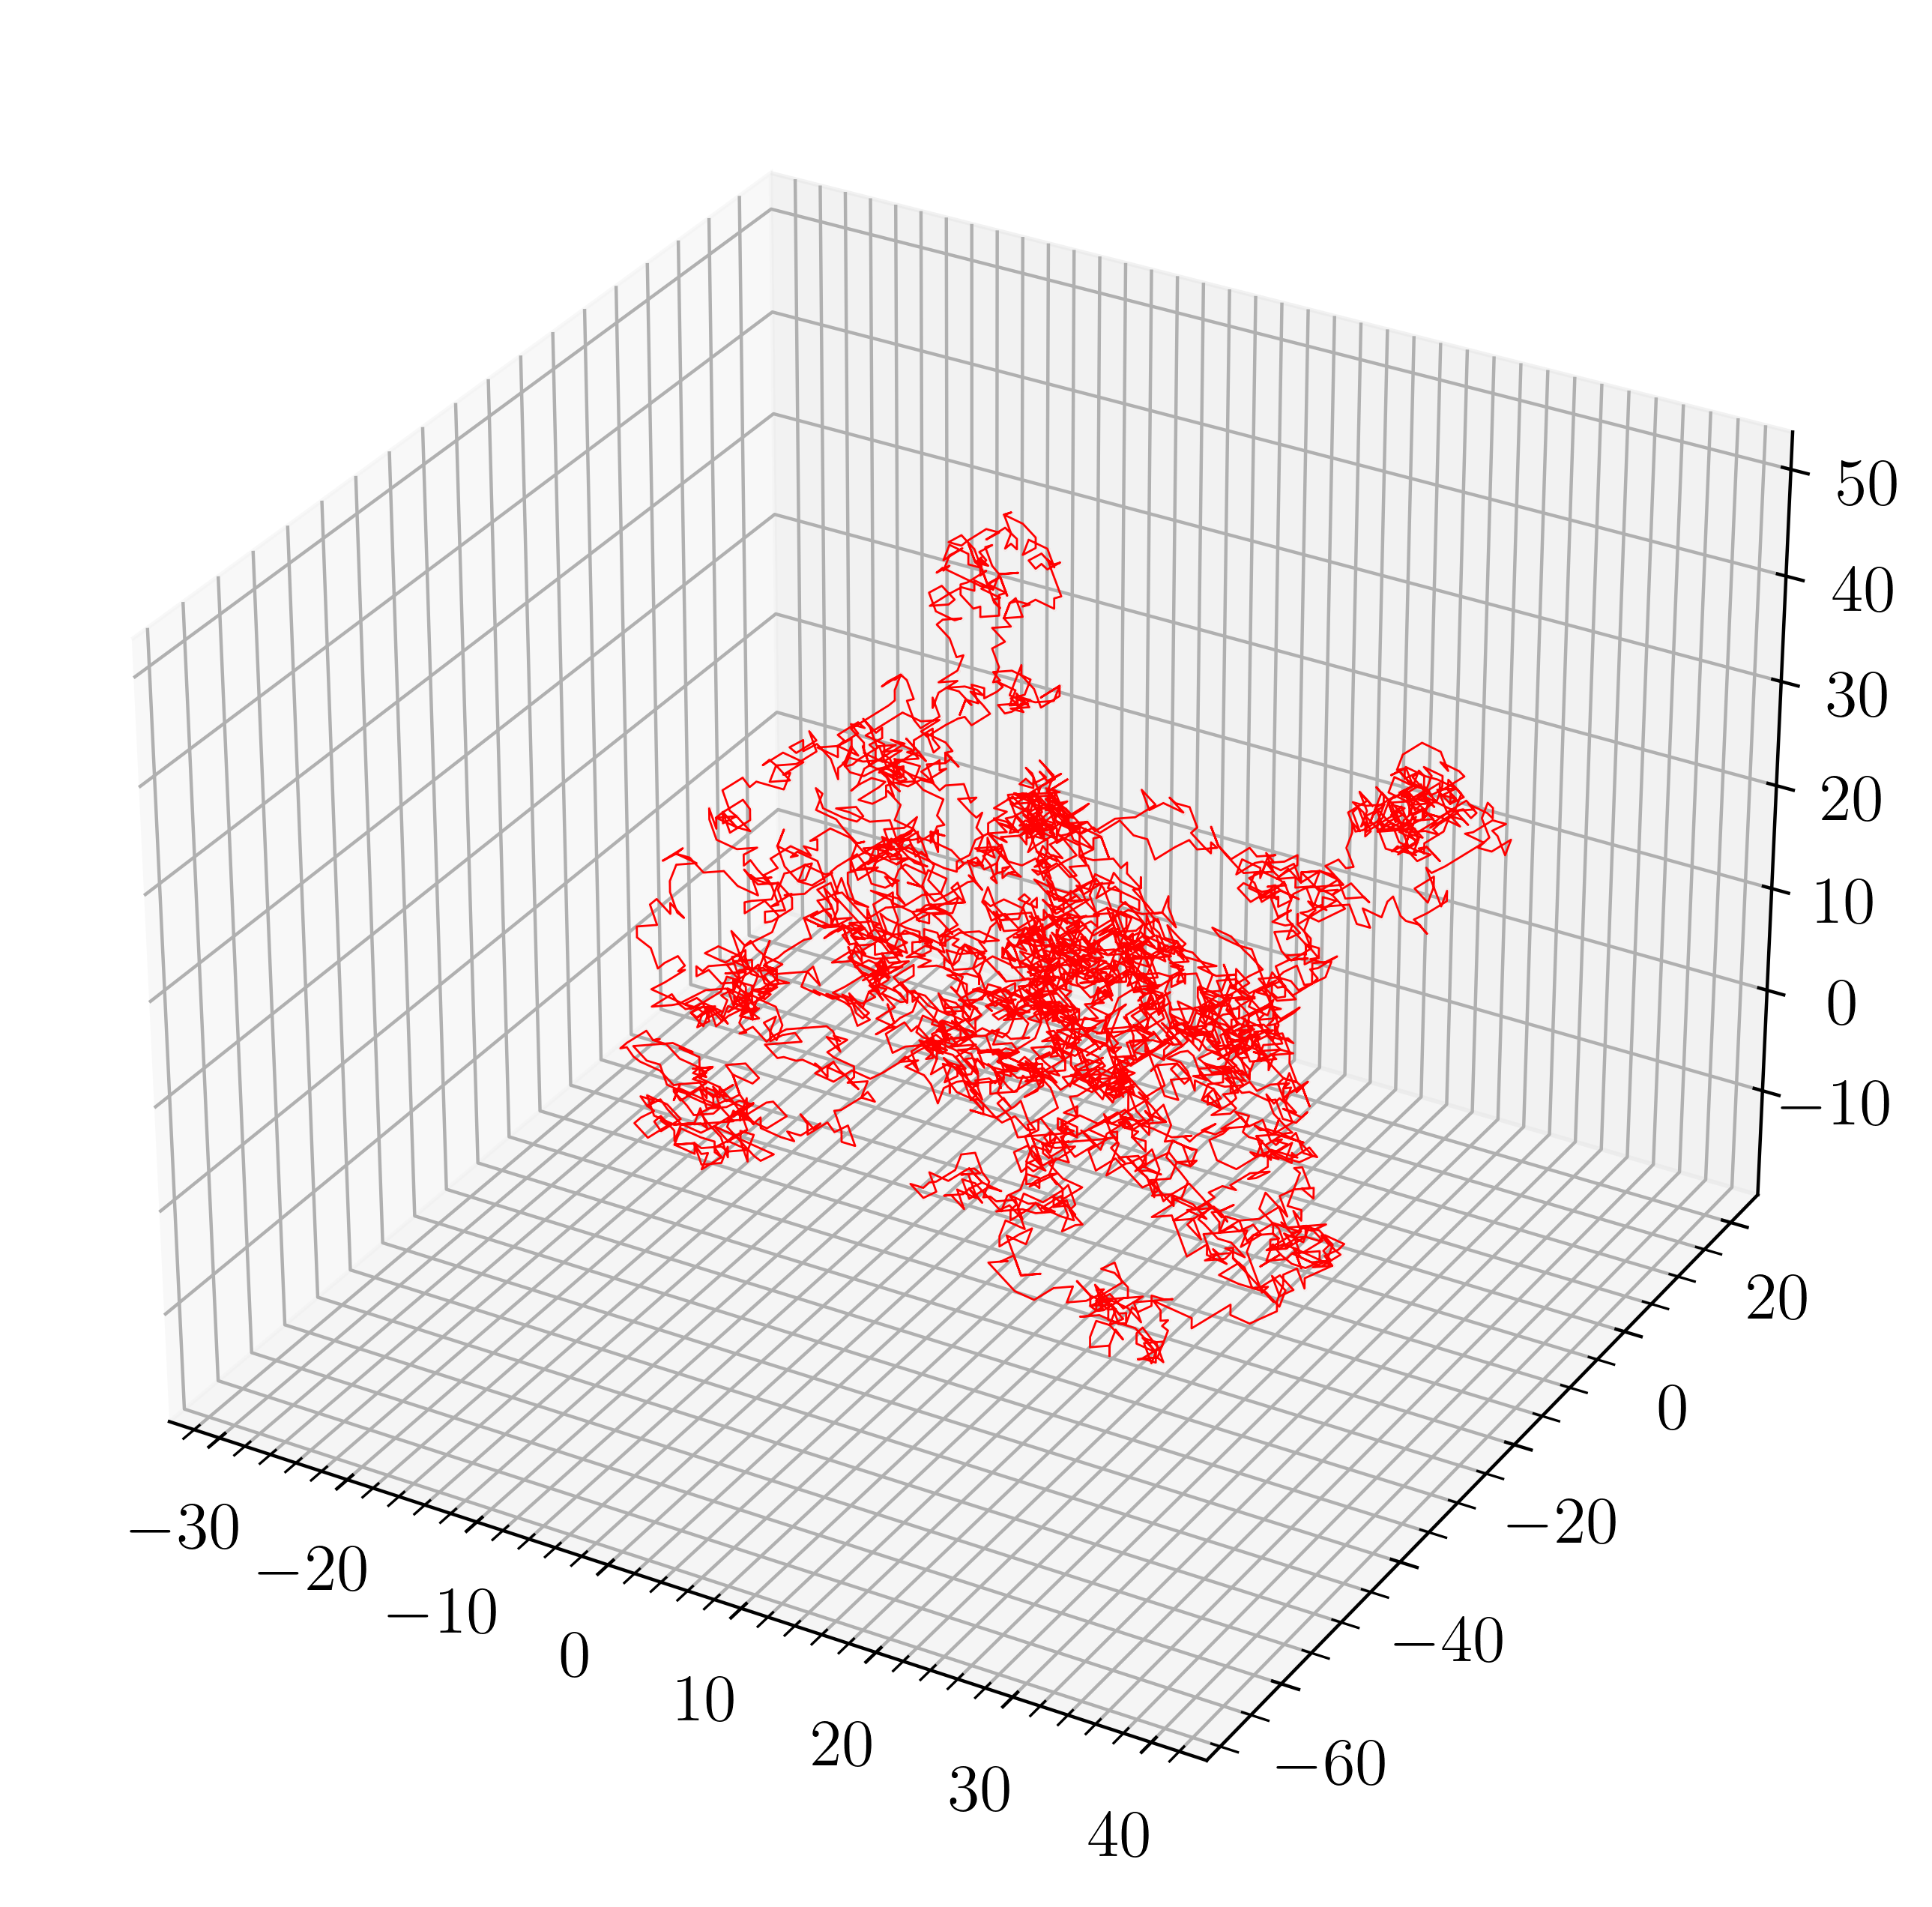
\includegraphics[width=0.6\textwidth]{tarefa-3/exemplo-random-walk-3D.png}
  \caption{Ilustração de uma caminhada aleatória em 3D.}
\end{marginfigure}

As mudanças do código \verb|DLA-2D.f| para o \verb|DLA-3D.f| consistem em adição de mais uma
coordenada e assim como antes também há um arquivo \verb|run.sh| para executar algumas \emph{seeds}
pre-determinadas (no próprio arquivo).

Segue abaixo o código que implementa a dinâmica do \emph{DLA-3D}:

\begin{marginfigure}
  \centering
  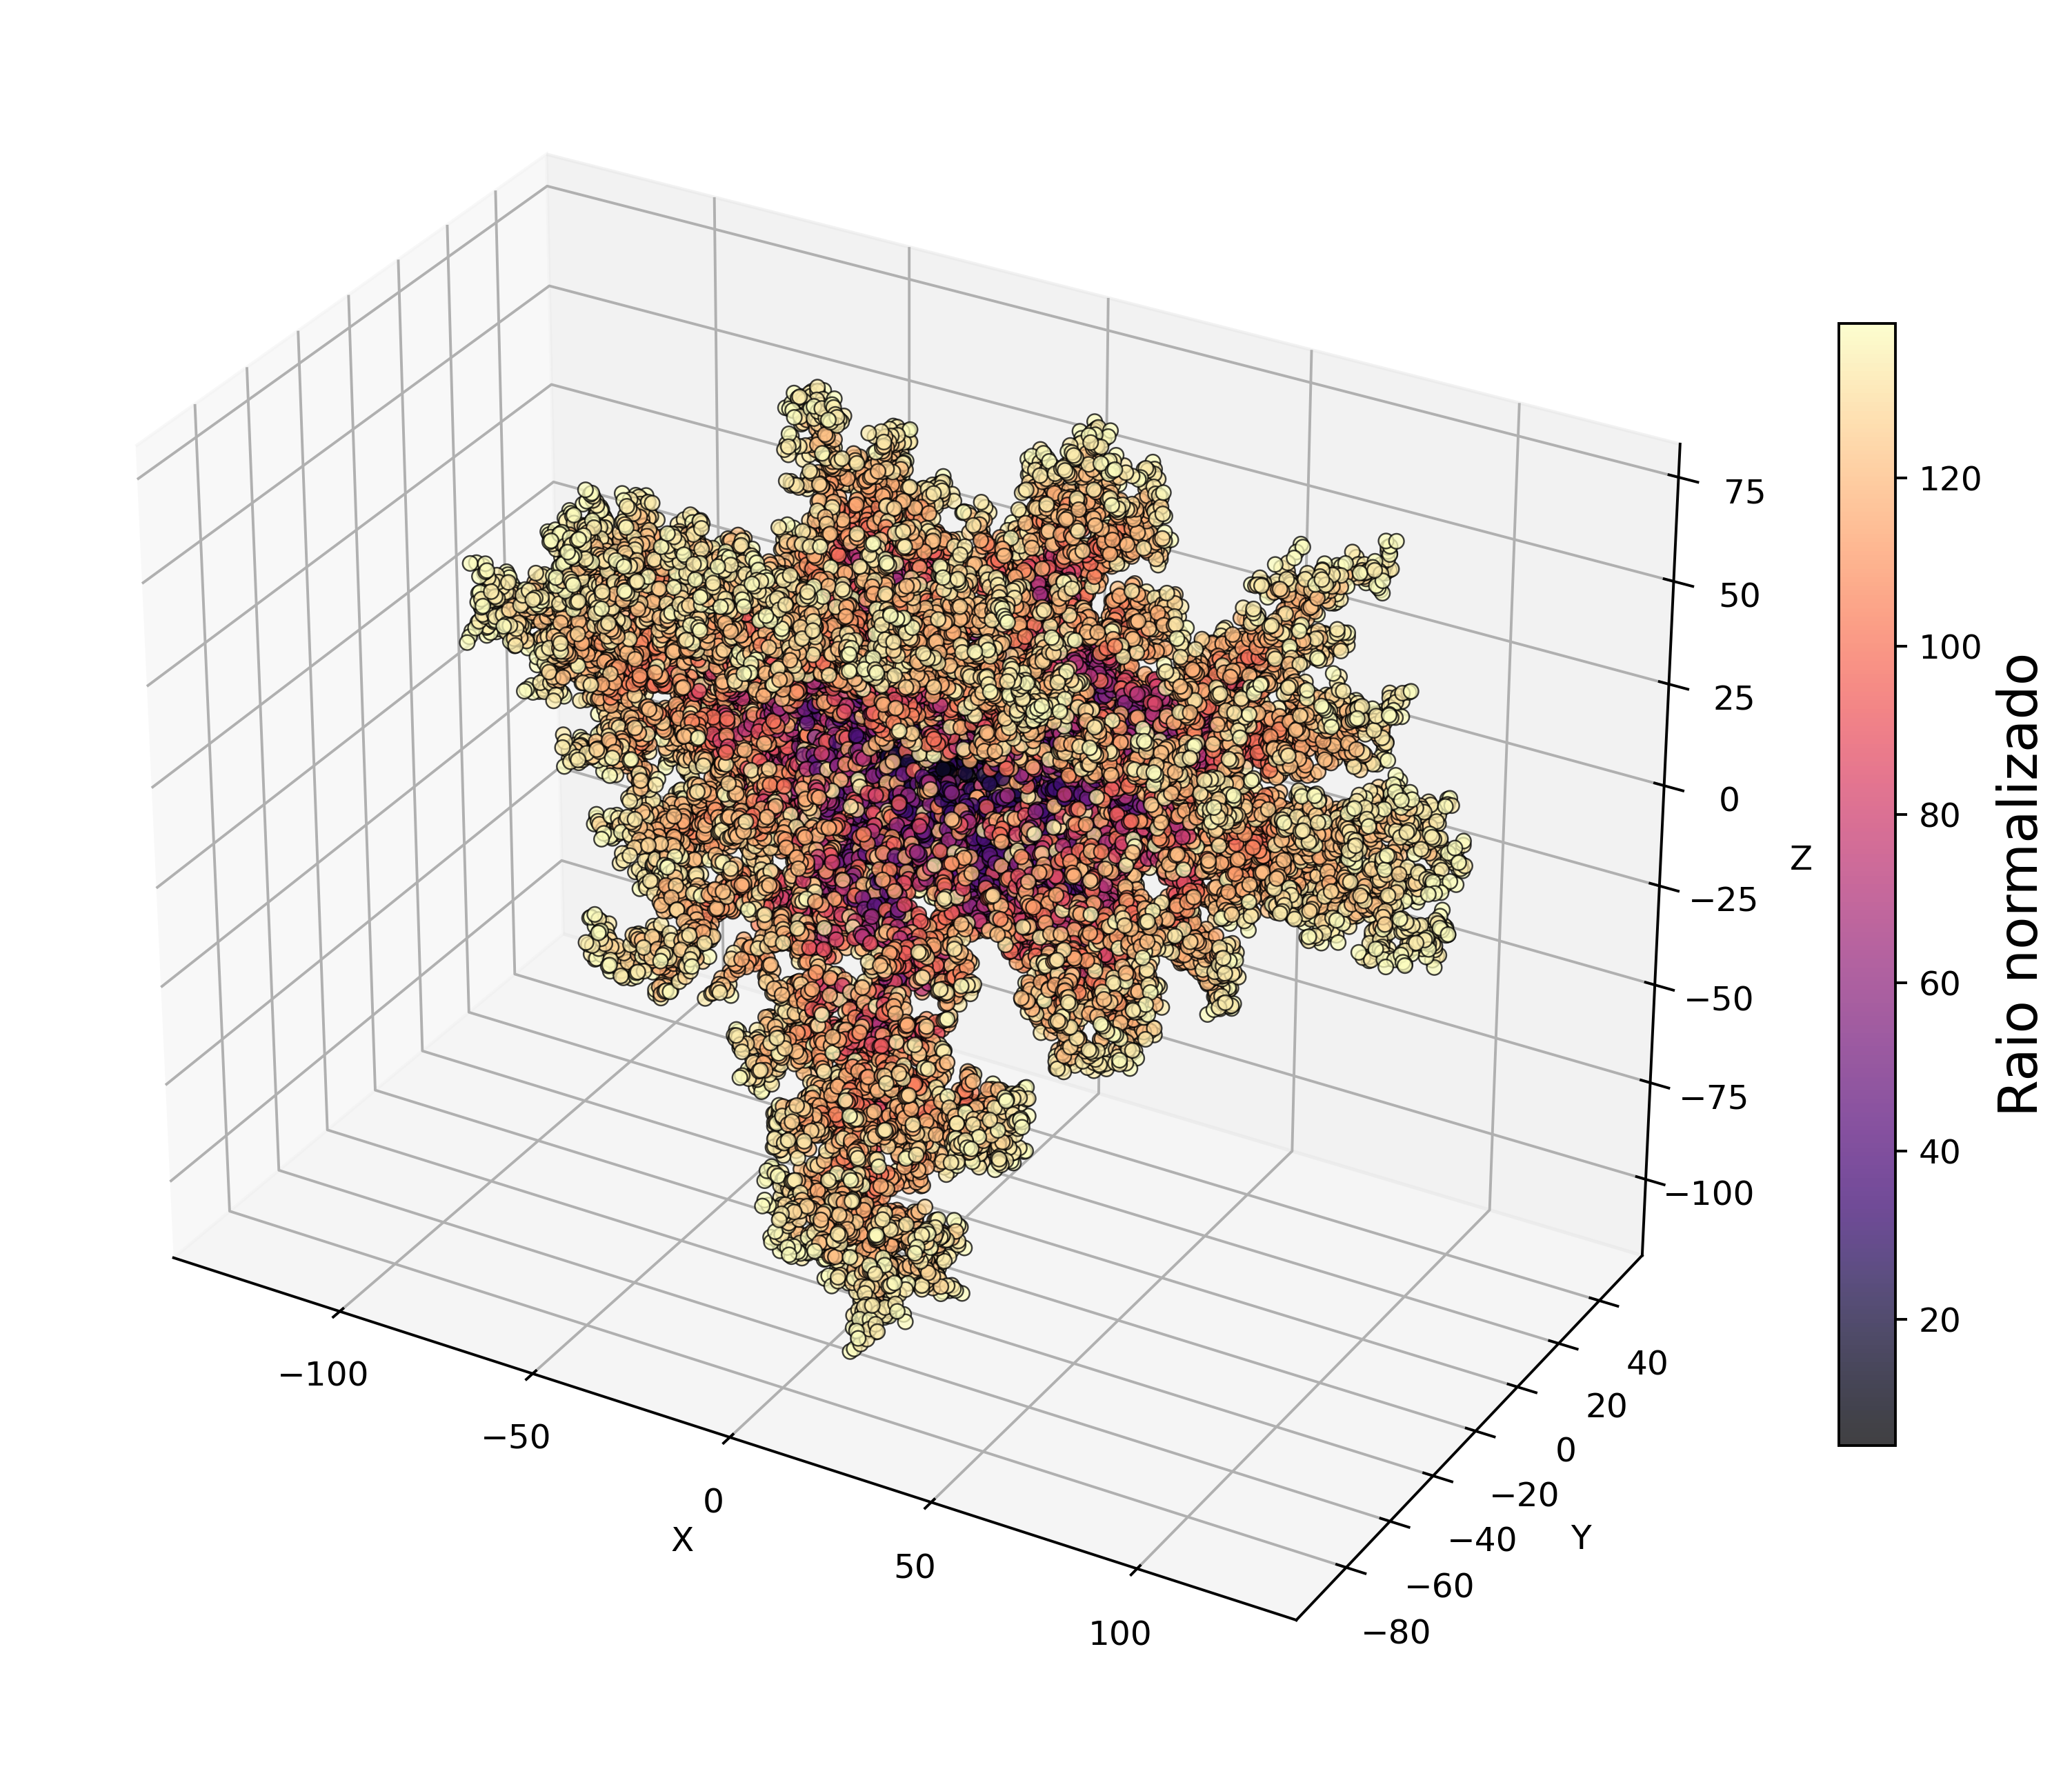
\includegraphics[width=0.75\textwidth]{tarefa-3/DLA_3D-grafico-1.png}
  \caption{SEED = 51}
  \label{fig:dla_3d_seed1}
\end{marginfigure}

\begin{marginfigure}
  \centering
  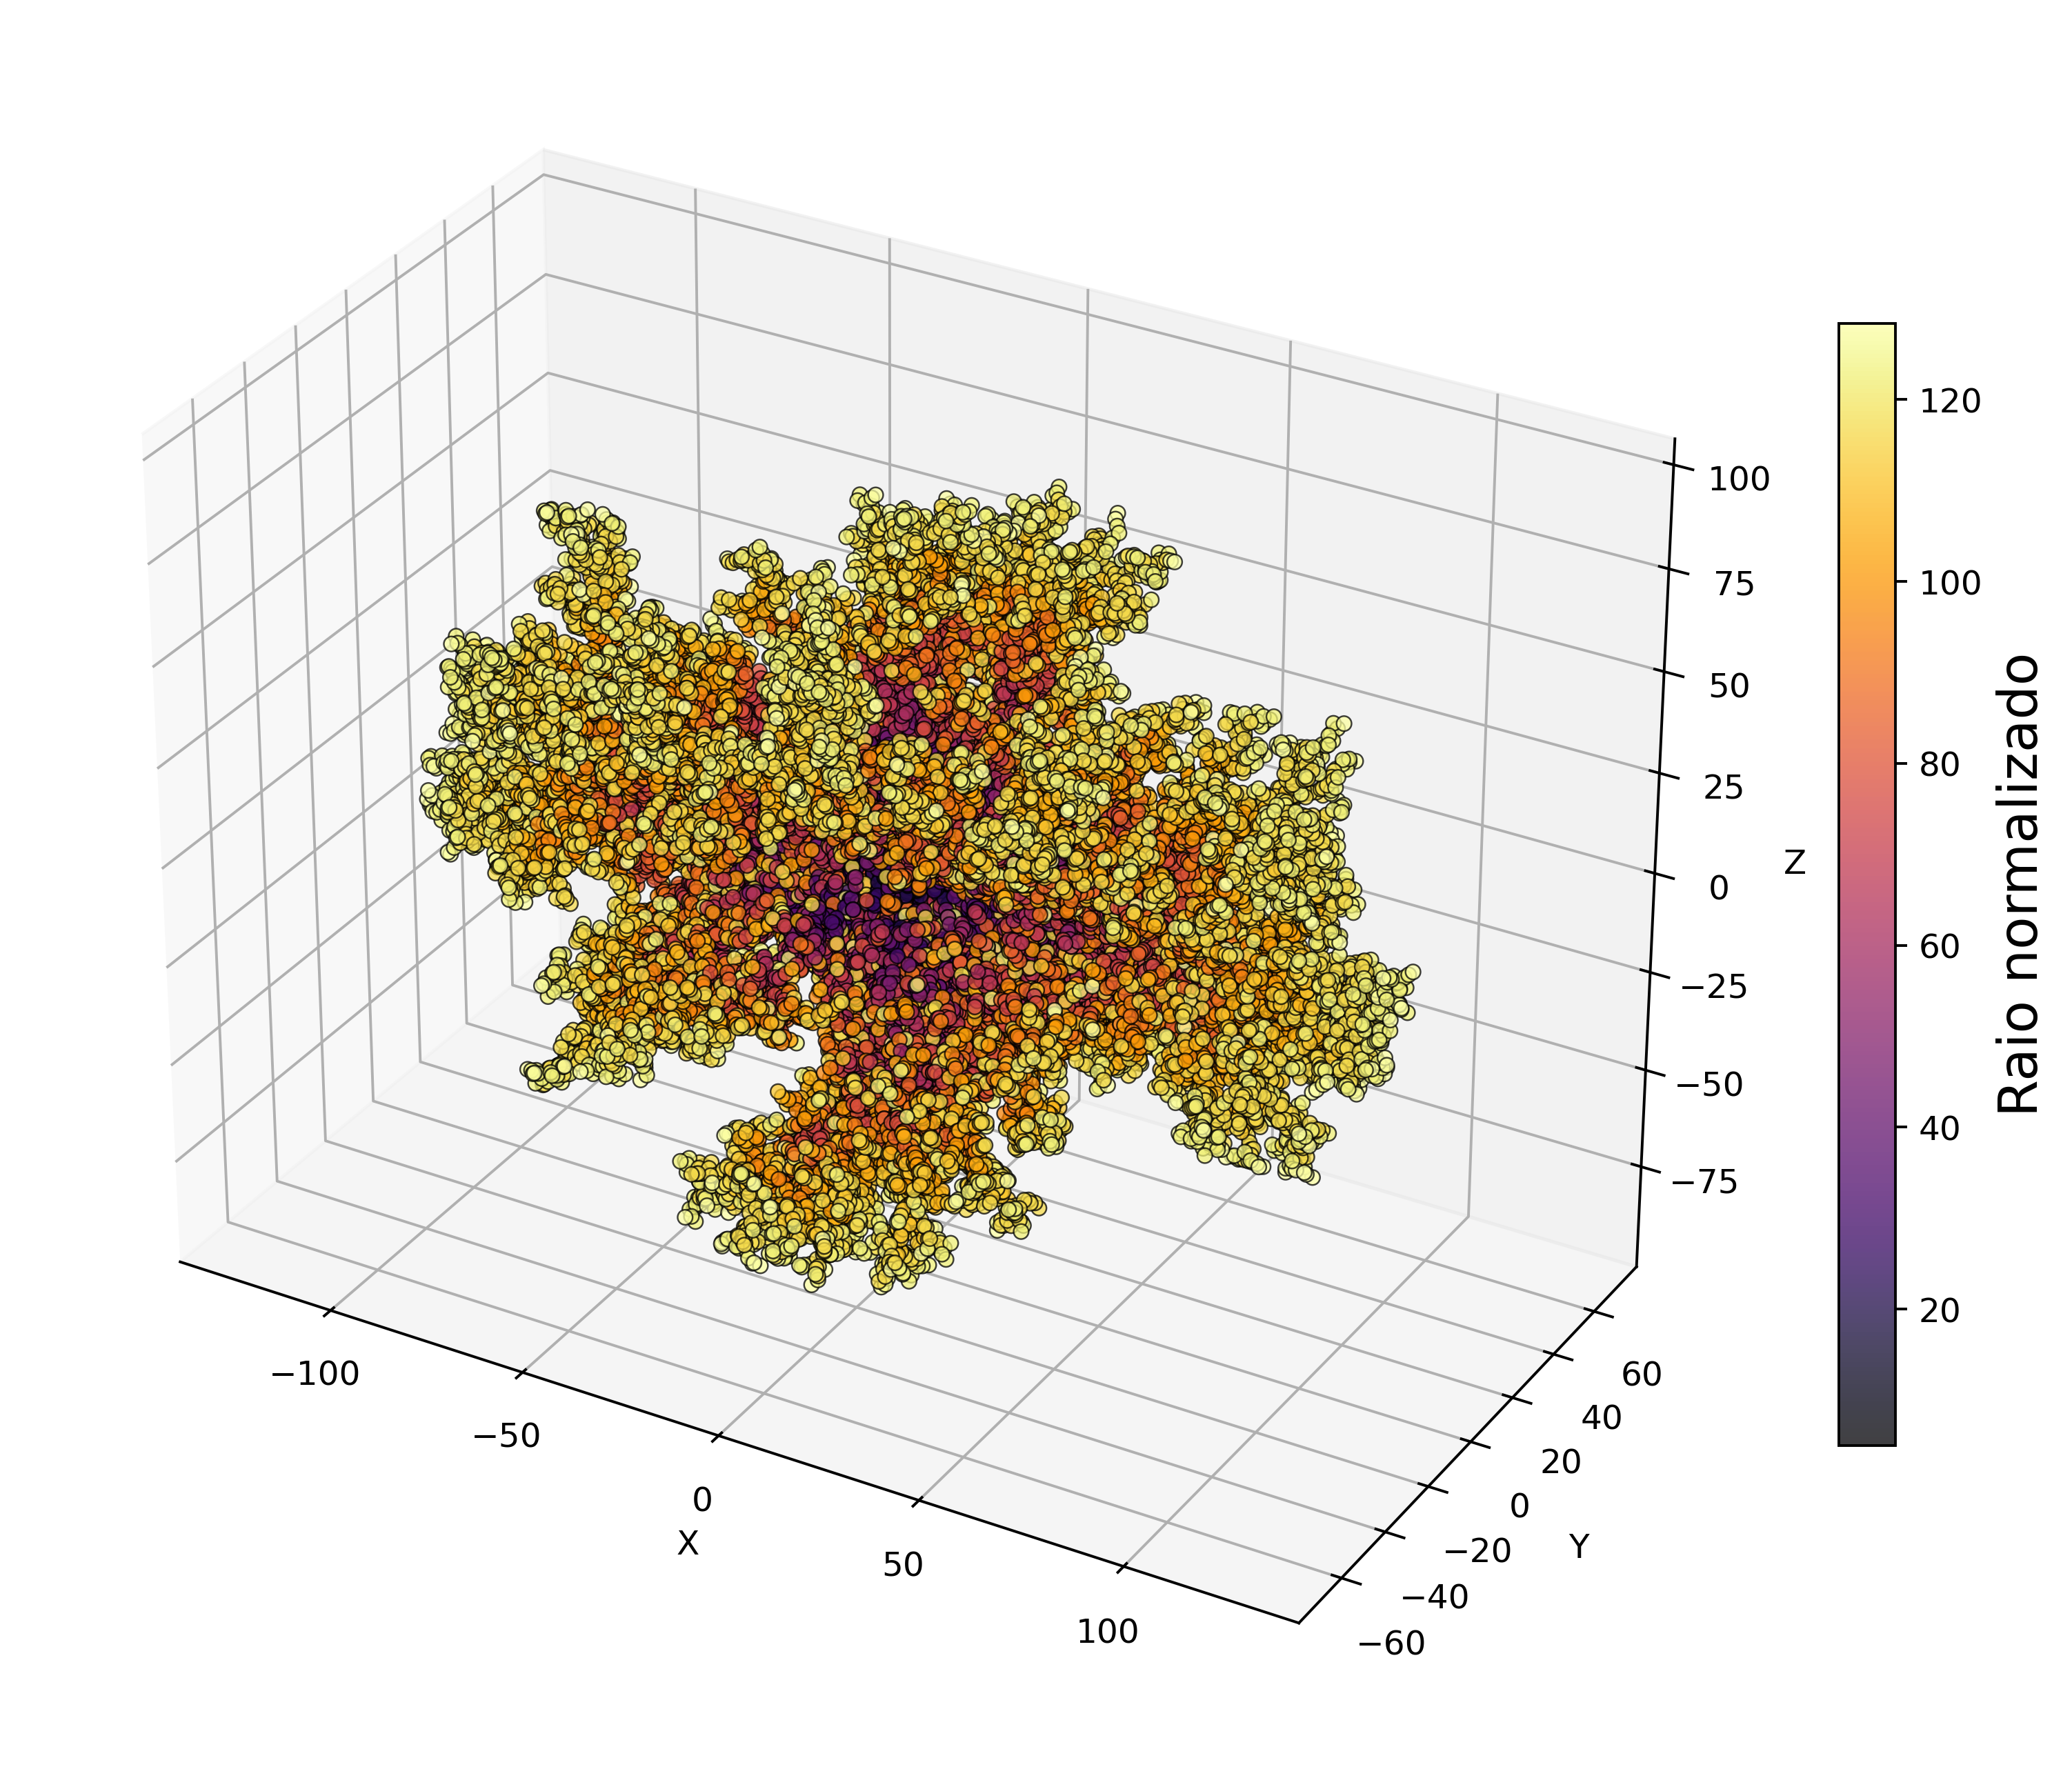
\includegraphics[width=0.75\textwidth]{tarefa-3/DLA_3D-grafico-2.png}
  \caption{SEED = 255}
  \label{fig:dla_3d_seed2}
\end{marginfigure}


\begin{marginfigure}
  \centering
  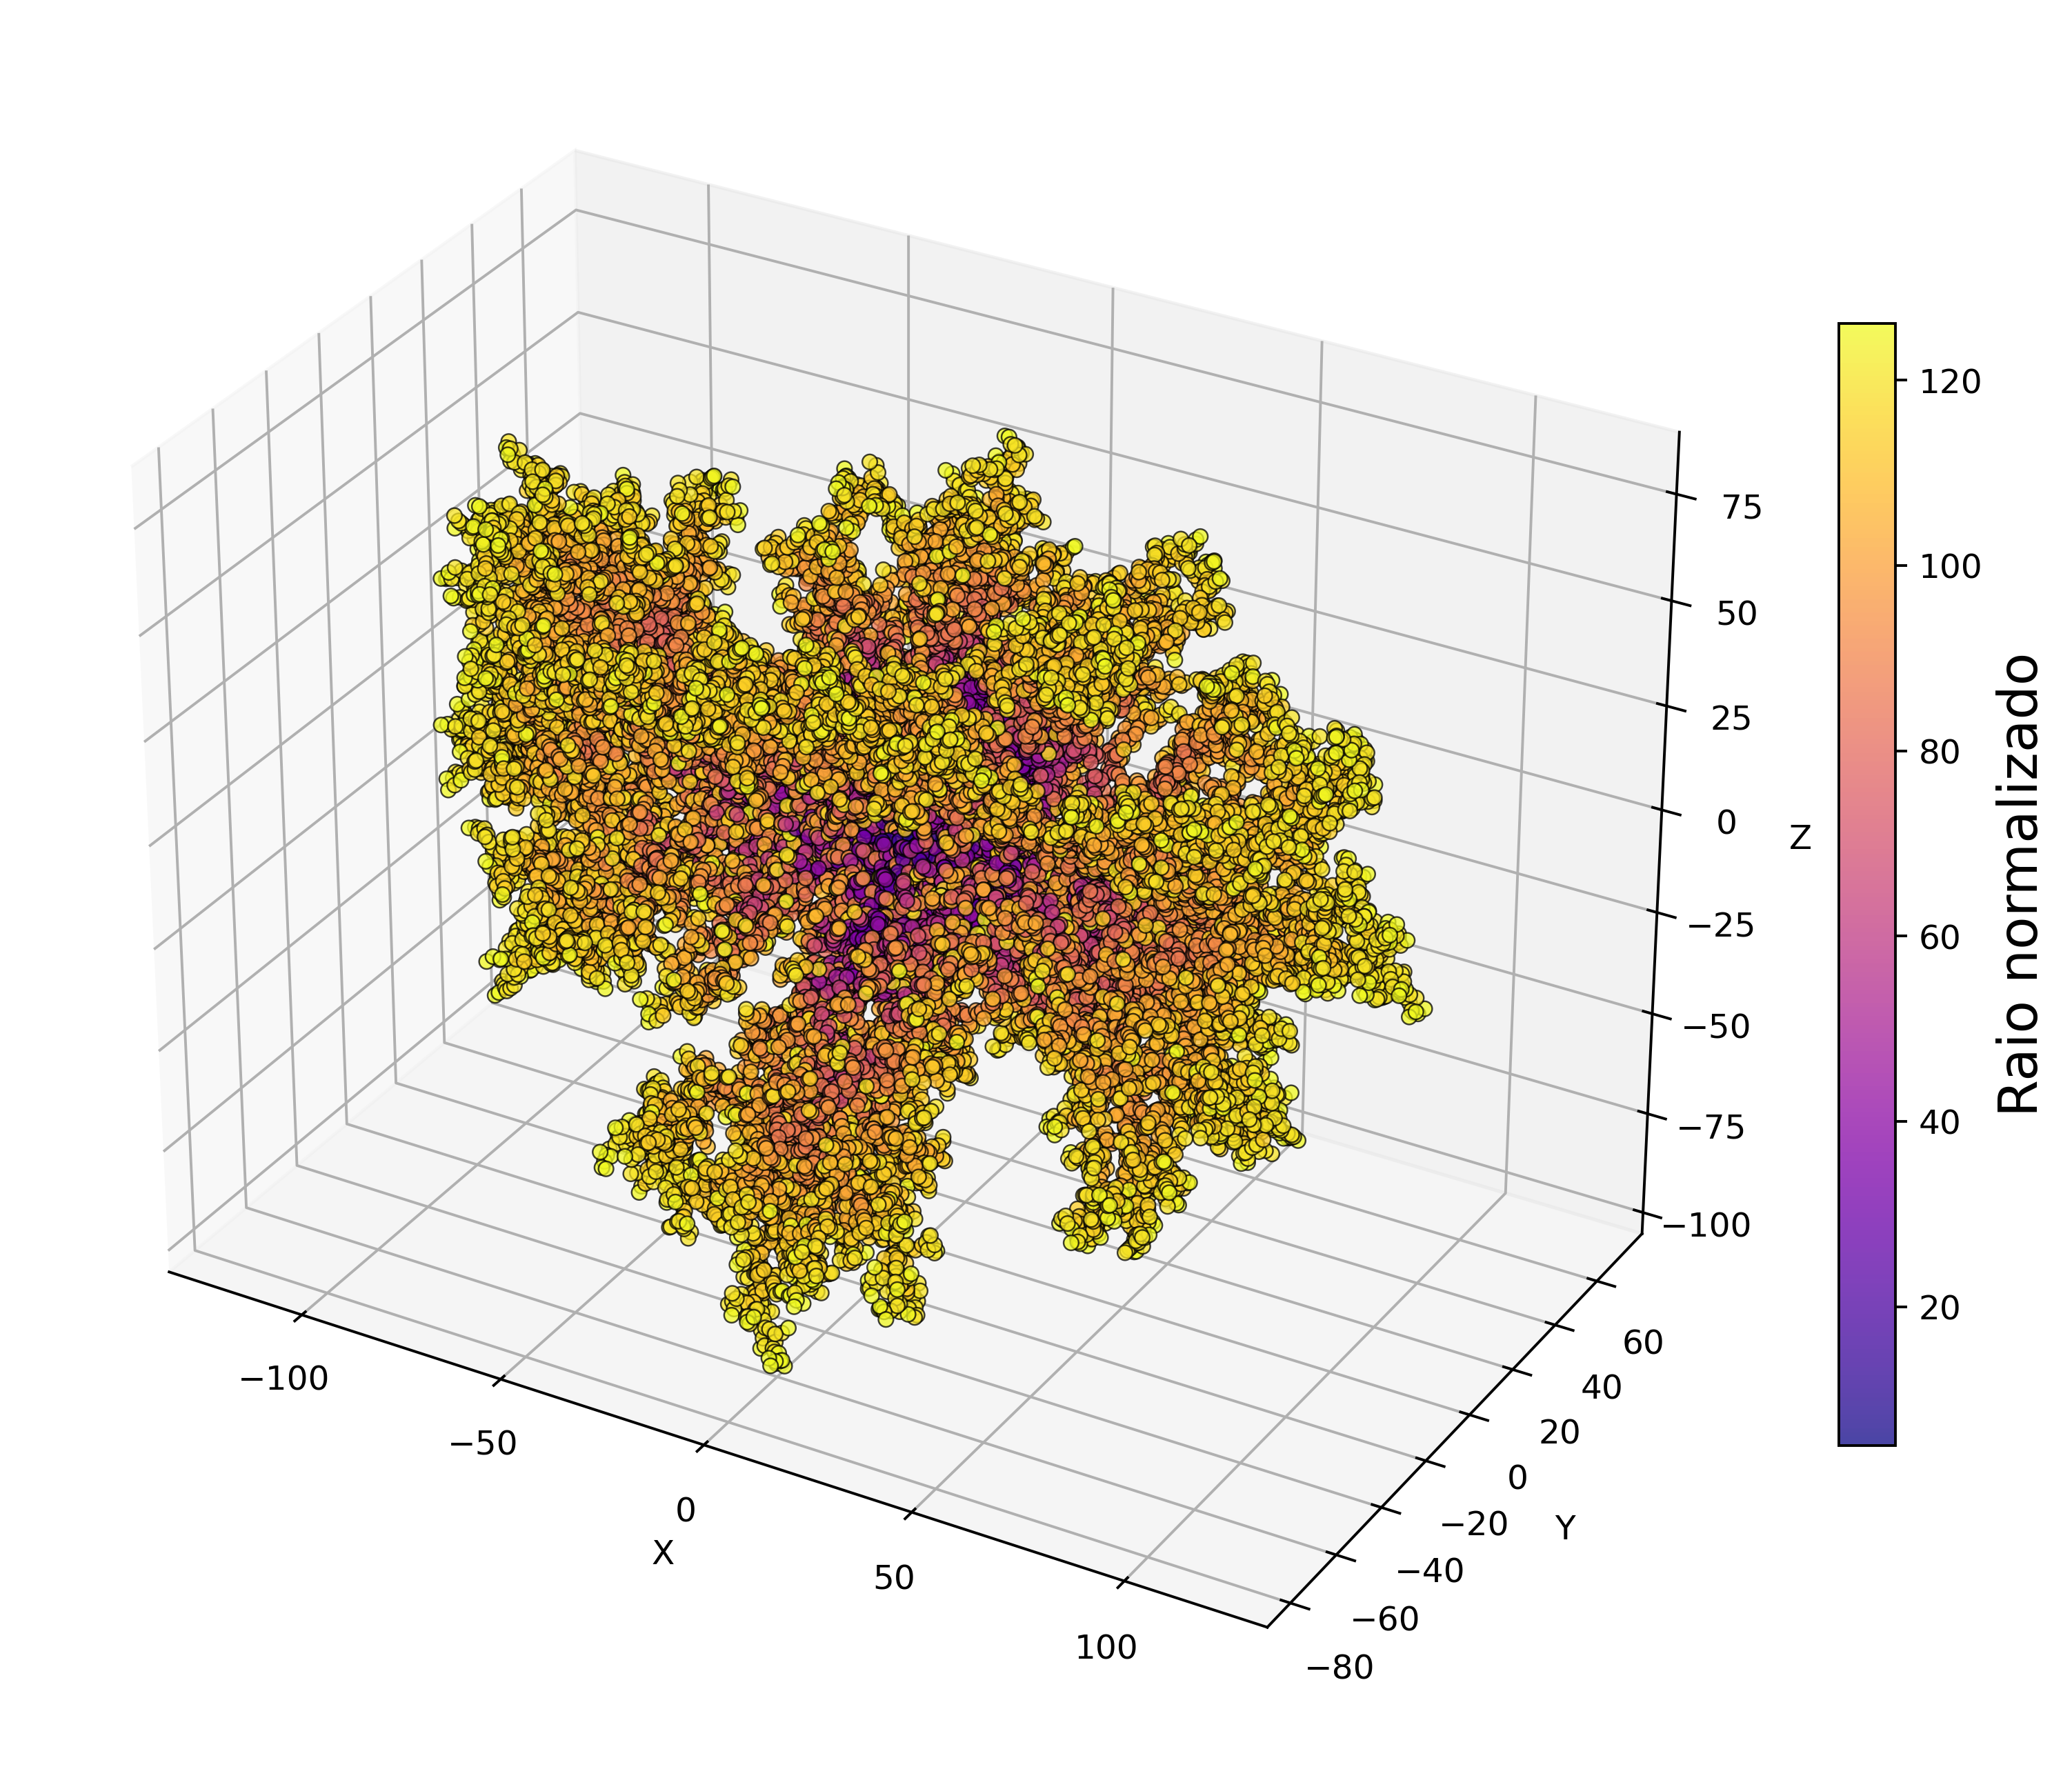
\includegraphics[width=0.75\textwidth]{tarefa-3/DLA_3D-grafico-3.png}
  \caption{SEED = 729}
  \label{fig:dla_3d_seed3}
\end{marginfigure}


\begin{minted}{fortran}
 !     Dinâmica DLA em 2D
!     Para cada partícula:
!     - Gera posicao inicial aleatoria.
!     - Aplica dinâmica de random walk.
!     - Ao agregar novas celulas armazena a posição e raio atual à um
!     arquivo de dados.
!     Parâmetros:
!     Np -> numero de particulas
      subroutine DLA_3D(Np, iseed)
      implicit integer (x-x, y-y, z-z)
      parameter(N = 500)
      dimension lattice(-N:N, -N:N, -N:N)

!     semente inicial
      lattice(0, 0, 0) = 1
     
      rnd = rand(iseed)
      
      R_in = 5.0
      R_f = 1.5 * R_in


      open(1, file="saida-dla.dat")
      open(2, file="saida-contagem.dat")

      nparts = 0
      do i = 1, Np

         x = 0
         y = 0
         z = 0

         print *, "Particle #", i

         call generate_random_particle(R_in, x, y, z) 

!        print *, "r = ", R_in
         s = 0
         touched = 0

         do while(touched == 0) 

            call random_step(x, y, z) 

            d = sqrt(real(x**2+y**2+z**2))
!     Captura celula ao redor da posição atual se houver
            do k = -1, 1
               do j = -1, 1
                  do l = -1, 1
!     Checagem de borda
                     if(abs(x) < N .and. abs(y) < N)then
                        s = s + lattice(x+k, y+j, z+l)
                     end if
                  end do
               end do
            end do
!     Adiciona nova celula, atualiza raio
            if (d >= R_f) then
               touched = 1
            else if(s >= 1) then
               touched = 1
               lattice(x, y, z) = 1

               nparts = nparts + 1
!     Salva o cluster, particulas e raio
               write(1, *) x, y, z, R_in
               write(2, *) R_in, nparts
               if(d > R_in) then
                  R_in = d + 5
                  R_f = 1.5 * R_in
               end if
            end if
         end do
      end do
      close(1)
      close(2)
      end subroutine DLA_3D
!     Gera uma partícula em uma posicao aleatoria
!     dado um raio inicial R_in
      subroutine generate_random_particle(R_in, x, y, z) 
      implicit integer (x-x, y-y, z-z)
      parameter(pi = acos(-1e0))

      rnd_val1 = rand()
      rnd_val2 = rand()

      theta = 2 * pi * rnd_val1
      phi = 2 * pi * rnd_val2

      x = int(R_in * cos(theta)*cos(phi))
      y = int(R_in * sin(theta)*sin(phi))
      z = int(R_in * sin(theta))

      end subroutine generate_random_particle

!     Dinâmica das particulas.
!     Executa random-walk até que: atinge uma celula ocupada
!     Parametros:
!     posicao x, y
      subroutine random_step(x, y, z)
      implicit integer(x-x,y-y,z-z)

      x = x + floor(rand()*3) - 1
      y = y + floor(rand()*3) - 1
      z = z + floor(rand()*3) - 1

      end subroutine random_step
\end{minted}

As imagens(\ref{fig:dla_3d_seed1})(\ref{fig:dla_3d_seed2})(\ref{fig:dla_3d_seed3}) dos aglomerados
em 3D foram adicionados apenas como fins de ilustração. No entando usando
alguns software interativos pode ser útil ter uma representação 3D do corpo final.


Assim antes estamos interessados em observar o crescimento de numero de pontos para um dado raio.
O resultado obtivo está na figura abaixo (\ref{fig:fig_n_r_fractal_3d}). 

\begin{figure*}[h!]
  \centering
  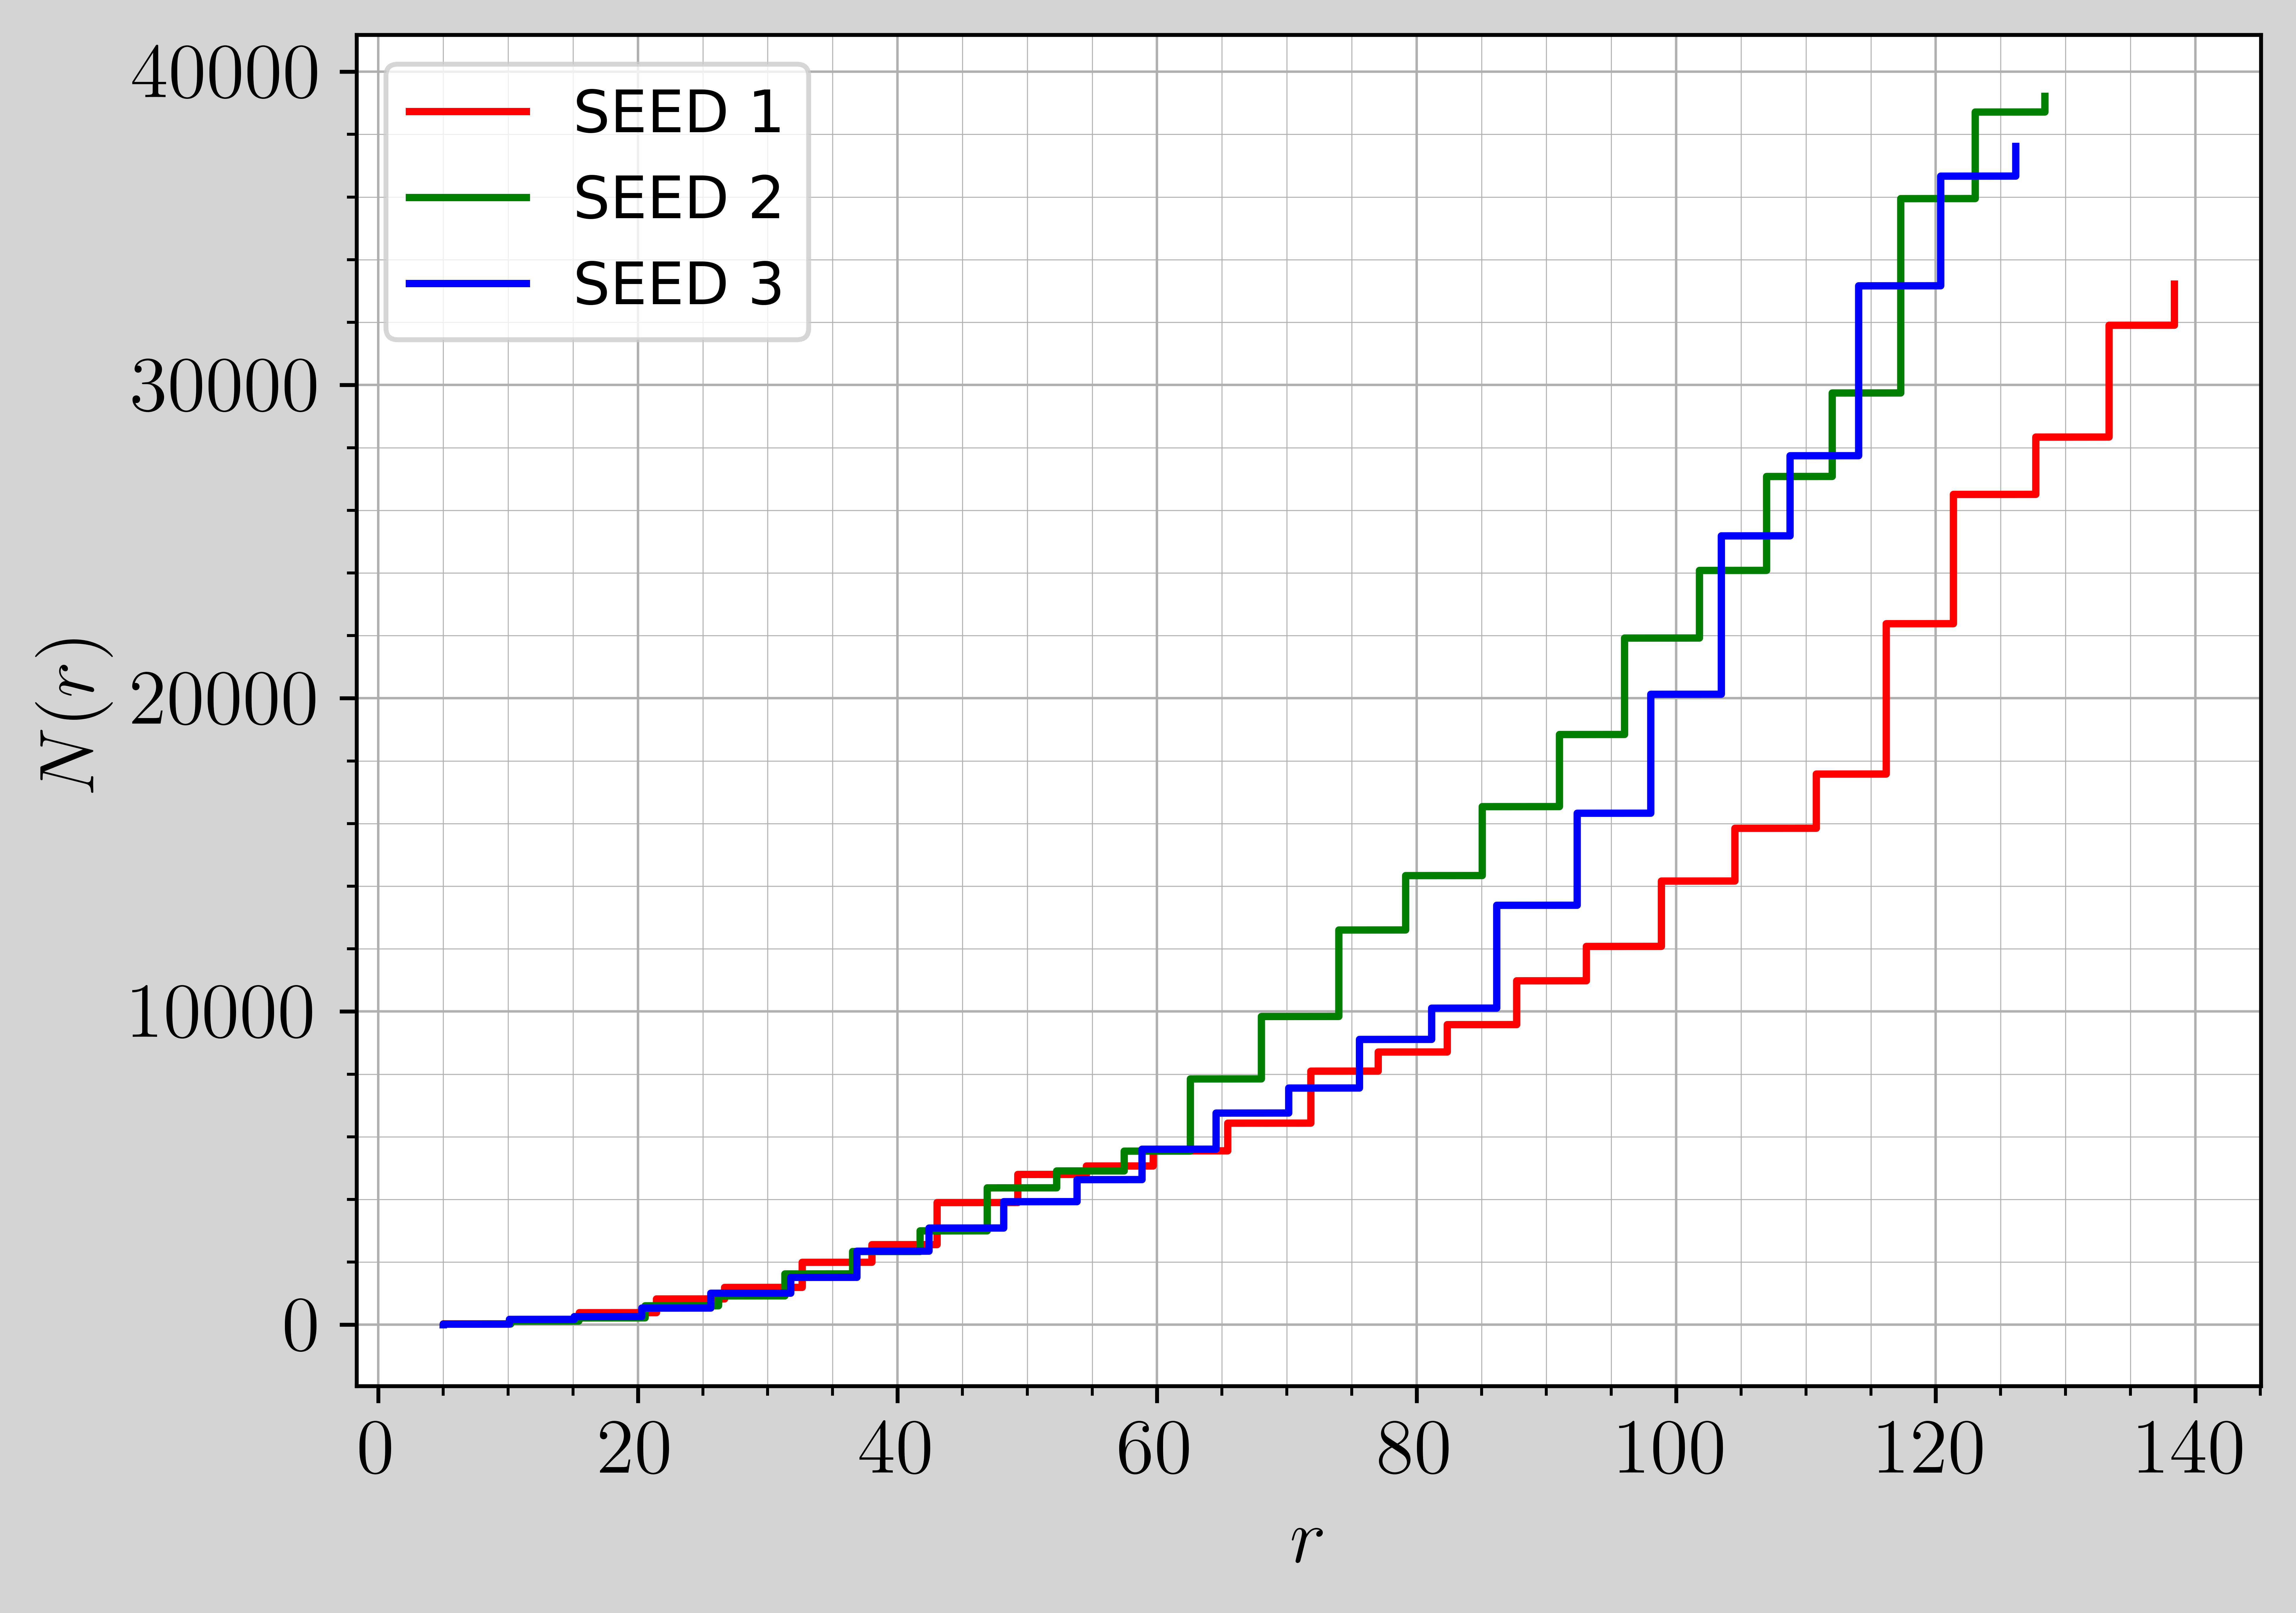
\includegraphics[width=0.6\textwidth]{tarefa-3/tarefa-3-graf-pontos-raio.png}
  \caption{Número de pontos $N(r)$ em função do raio $r$.}
  \label{fig:fig_n_r_fractal_3d}
\end{figure*}


Fazendo novamente a linearização e regressão linear obtemos os coeficientes que determinam
a dimensão fractal para as simulações.

\begin{figure*}
  \centering
  \includegraphics[width=0.7\textwidth]{tarefa-3/tarefa-3-graf-regressao-linear-dimensao-fractal.png}
  \caption{Estimando dimensão fractal $d_f$.}
  \label{fig:fig_fractal_3d}
\end{figure*}


Pela (\ref{fig:fig_fractal_3d}) obtemos \( d_f =  2,08 \), \( d_f = 2,47 \) e \( d_f = 2,49 \)
para as \emph{seeds} de número aleatório utilizadas.
Não foram feitas análises mais detalhadas dos valores obtidos como médias ou desvio padrão.


\clearpage
\section{Efeito corona}

Nessa tarefa aplicamos o modelo de crescimento implementado na tarefa dois para \emph{DLA-2D}
em condições iniciais nas quais o comportamento do sistema é parecido o efeito corona observado
em fios condutores.

As únicas alterações realizadas ao código \verb|tarefa-2/DLA_2D.f| foram as condições iniciais
e geração de pontos aleatórios. Adotamos sistema com partículas situadas em todas posição \( x \)
para dado vertice \( y \), que para simulação foi adotado sendo \( y = 0\). Os pontos aleatórios que
realizam movimento browniano são gerados como antes à uma distância fixa, mas não são pontos
aleatórios no plano ou espaço, ao invés de angulo adotamos um espaço retangular no qual o ponto pode
ser gerado.


Segue abaixo o código da segunda tarefa alterado para simular o efeito corona:


\begin{minted}{fortran}
!     Efeito corona
!     código da tarefa-2 : dla_2d
!     com adaptação nas condições iniciais e tamanho
!     do lattice em Y.
      implicit integer (x-x, y-y)
      parameter(N = 800)
      dimension lattice(-N:N, 0:5000)
      Np = 80000
      read(*, *) iseed
      call srand(iseed)
      lattice = 0
      open(1, file="saida-dla.dat")
!     semente inicial
      do i = -N, N
         lattice(i, 0) = 1
         write(1, *) i, 0
      end do
      Y_in = 5
      Y_f = 1.5 * Y_in
      do i = 1, Np
         touched = 1
         print *, "Particle #", i
!     Gera uma particula em um ponto aleatorio.
         x = (2 * N * rand()) - N
         y = R_in
         do while(touched == 1) 
!      Passo aleatorio
            x = x + floor(rand()*3) - 1
            y = y + floor(rand()*3) - 1
!     Conta numero de vizinhos proximos
            do j = -1, 1
               do k = 0, 1
                  sum = sum + lattice(x + j, y - k)
               end do
            end do
            if(x >= N .or. x < -N .or. y > R_f) then
               touched = 0
            else if (sum > 0) then
               lattice(x, y) = 1
               write(1, *) x, y
               touched = 0
               sum = 0
               if(y == R_in) then
                  R_in = R_in + 5  
                  R_f =  R_in * 1.5
               end if 
            end if
         end do
      end do
      close(1)
      end
\end{minted}


\begin{figure*}
  \centering
  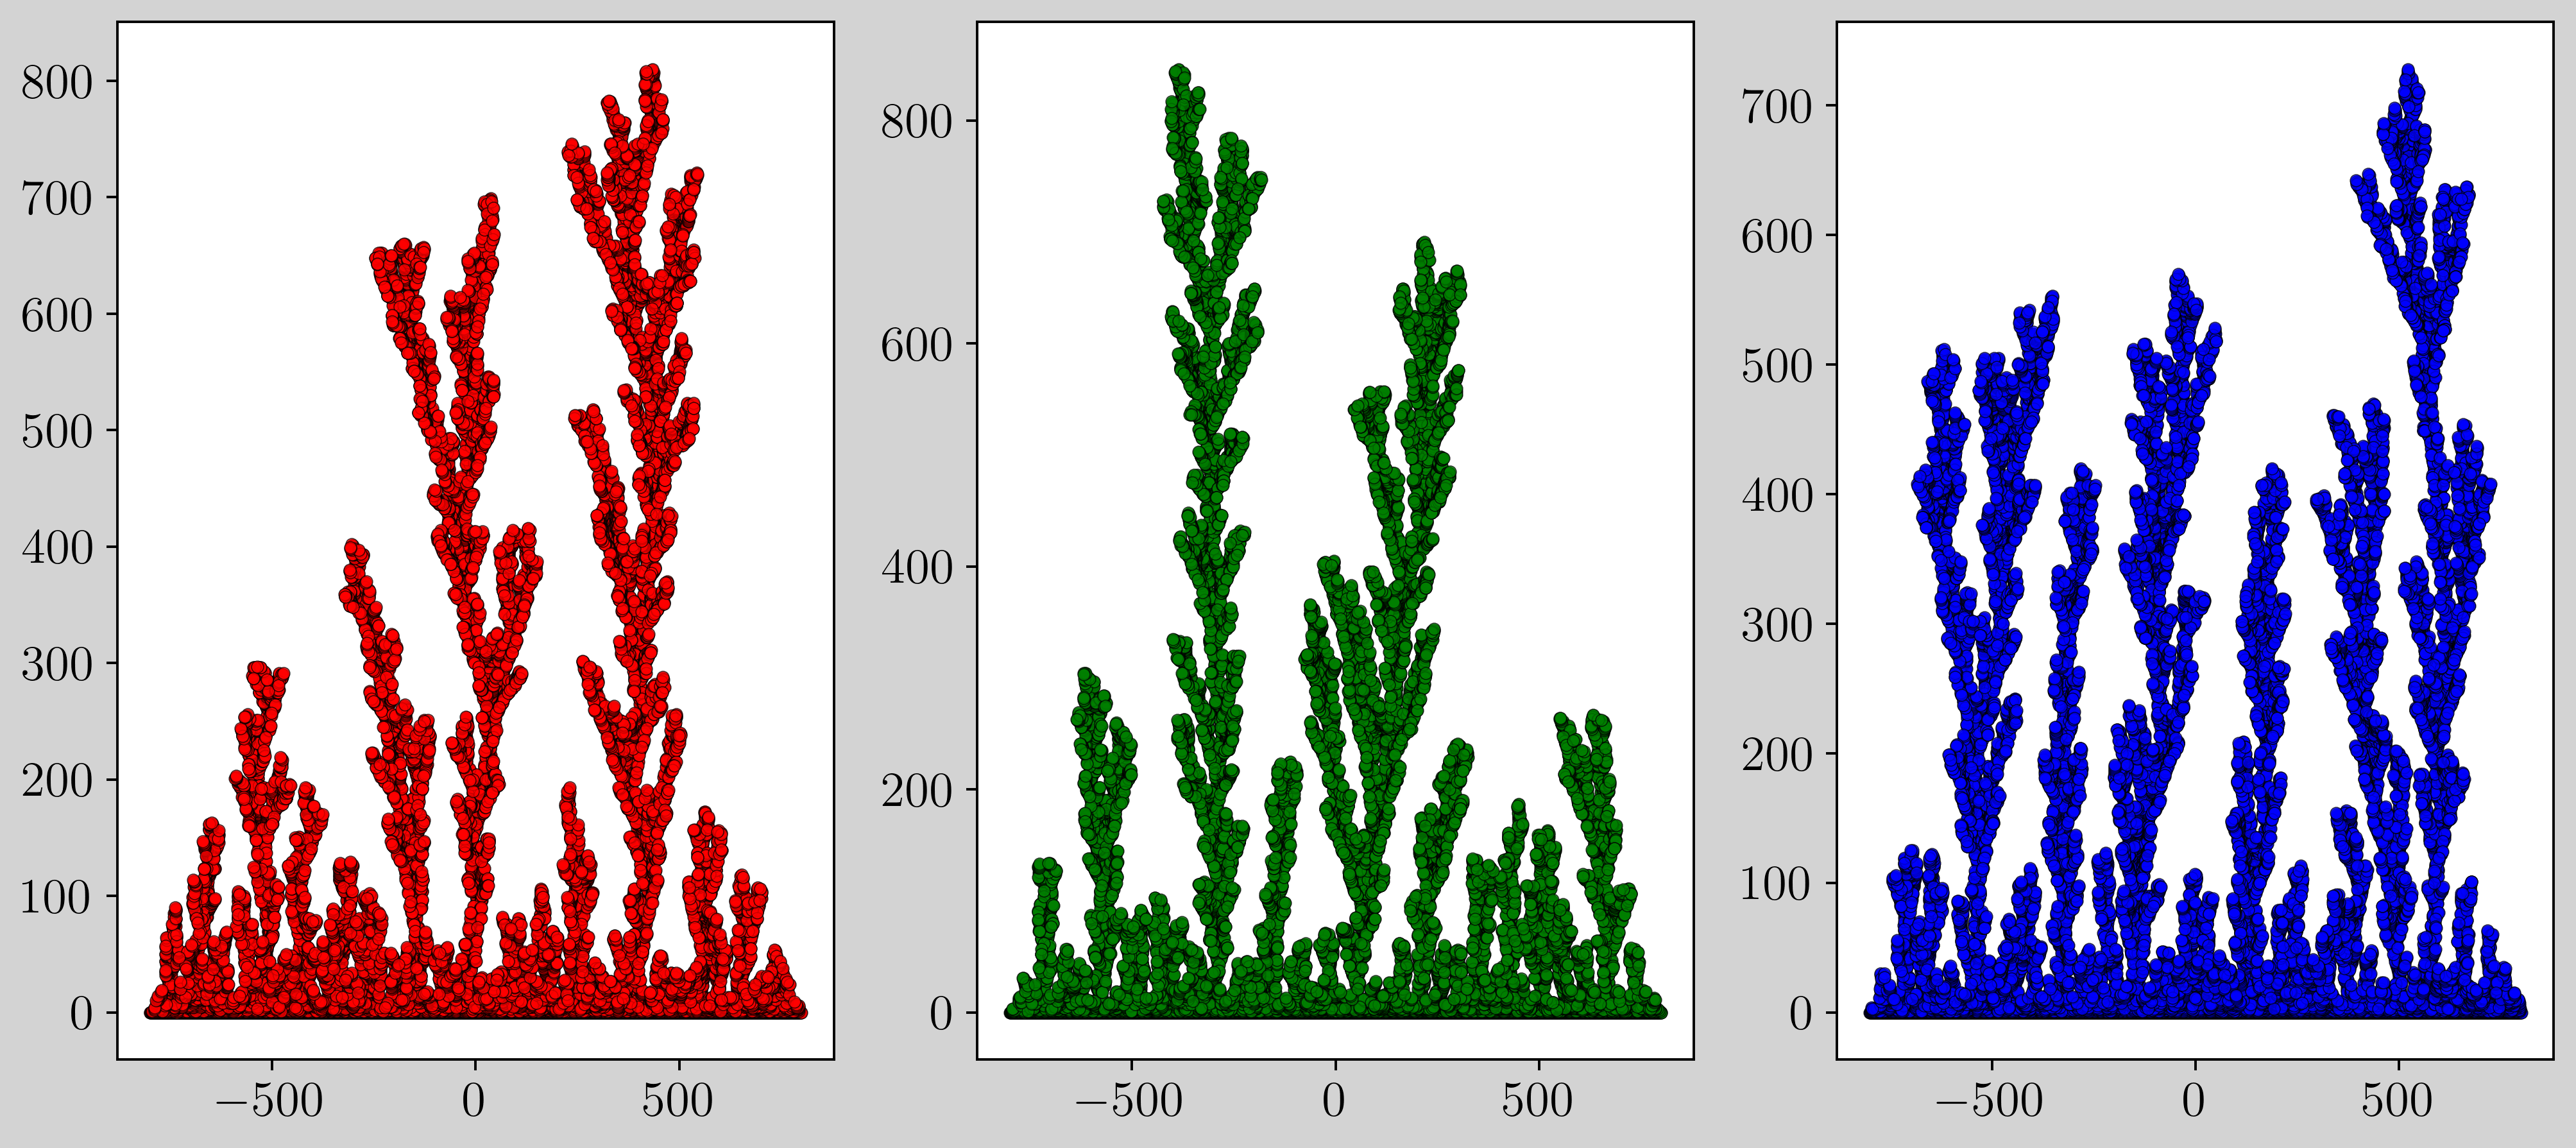
\includegraphics[width=0.7\textwidth]{tarefa-4/efeito-corona.png}
  \caption{Simulações do Efeito Corona para algumas \emph{seeds} quaisquer.}
\end{figure*}


\clearpage
\section{Revoluções populares}

A última, e mais desafiadora, simulação realizada é a de um modelo simples de ``revolução popular''
utilizando as ideias do \emph{diffusion limited agregation}.

Nesse modelo geramos por um processo de Bernoulli um número consideravel de partículas que
permanecem estáticas em seus respectivos sítios do reticulado.\footnote{Nota-se que o sistema
  poderia ser ainda mais complexo se aceitassemos todas partículas se movendo simultaneamente no
  reticulado.} Posicionamos então uma partícula que realizará random walk com a seguinte regra: ao
atingir um reticulado ocupado, ou seja, que tenha estado diferente de zero, deve adicionar essa
partícula ao aglomerado. Na simulação podemos limitar a contagem de passos que o ``processo
revolucionário'' vai realizar e observar o estado final do sistema após os $N$ passos.
É do nosso interesse observar a dependência do tamanho da dimensão fractal \( d_f \) com a
probabilidade \( p \) adotada no processo de Bernoulli. 


Foi adotada uma estratégia força bruta para realizar a simulação. Utilizando dois \emph{grids}
principais que representam o reticulado estático e o dinâmico, podemos partir da origem do sistema
com uma partícula e percorrer um raio $R$ em caminhada aleatória. Isto é, buscamos em torno de um
raio inicial se há partículas adjacentes, caso haja, são adicionadas e realizamos checagem do
tamanho atual do raio e a distância da partícula recem adicionada à o centro. Isso é semelhante ao
que foi feito na simulação do \emph{DLA-2D}.
Parte crucial da dinâmica é a realização do movimento
aleatório de todo o agregado. Para esse fim, temos um loop duplo em torno do raio $R$ atual no grid
dinâmico que análisa qual sítio do retículado possui uma partícula, caso haja, essa partícula
realiza um passo aleatório. Todas outras particulas do agregado realizam o mesmo passo.

Uma estratégia mais eficiente talvez seria buscar uma forma de realizar o movimento sem necessitar
analisar se há partículas em cada um dos sítios, utilizando alguma estrutura que salvasse estado
atual dos entornos. \footnote{Não consegui trabalhar nessa tarefa por tempo o suficiente para fazer
  um bom trabalho.}


Segue abaixo o código implementado para a simulação do modelo de revolução popular:


\begin{minted}{fortran}
      implicit integer (x-x, y-y)
      parameter(N = 1000)

      dimension lattice_static(-N:N, -N:N)
      dimension lattice_dynamic(-N:N, -N:N)
      dimension lattice_aux(-N:N, -N:N)

      dimension ipx(0:3)
      dimension ipy(0:3)
      parameter(ipx=(/1,-1,0,0/), ipy = (/0,0,1,-1/))

      p = 0.1

      open(1, file="output-fractal.dat")

      lattice_static(0, 0) = 0
      lattice_dynamic(0, 0) = 1

      call srand(33519)
      do i = -N, N
         do j = -N, N
            if (rand() <= p) then
               lattice_static(i,j) = 1
            end if
         end do
      end do
!     Dinamica
!     · Agragado pode aglutinar particulas por ate M passos
!     · Definimos um raio para o agregado pode buscar particulas adjacentes
!     · Para cada passo olhamos em volta do agragado, aglutinamos
!     · particulas, atualizamos raio e contamos # particulas no dado raio.
      k_radious = 5
      x = 0
      y = 0
      n_parts = 0
      ! passos 
      do m = 1, 3500
         print *, "STEP #", m
!     · Percorre raio em torno das coordenadas (x,y) do aglomerado.
         do i = -k_radious, k_radious
            do j = -k_radious, k_radious
               if(abs(x+i) < N .and. abs(y+j)<N) then
                  if(lattice_dynamic(x+i, y+j) == 1) then
!     · Percorre coordenadas adjacentes ao aglomerado.
                     do k = -1, 1
                        do l = -1, 1
!     · Aglomerado chocou com uma particula.
                           if(abs(i+k) < N .and. abs(j+l) < N) then
                              if(lattice_static(i+k,j+l)==1) then
                                 lattice_static(i+k,j+l) = 0
                                 lattice_dynamic(i+k,j+l) = 1
!     · Verifica se o raio ultrapassou do raio inicial k_radious:
                                 dist=sqrt(real((i+k-x)**2+(j+l-y)**2))
                                 if(dist >= k_radious) then
                                    k_radious = k_radious + 5
                                 end if 
                                 n_parts = n_parts + 1
!     · Escreve raio atual e numero de particulas 
                                 write(1, *)n_parts,(i+k)-x,(j+l)-y,dist
                              end if
                           end if 
                        end do
                     end do
                  end if
               end if
            end do
         end do
! Movimenta o aglomerado:
         x_step = 0
         y_step = 0
         ia = 4 * rand()
!     · Todas particulas do aglomerado estao dentro do raio k_radious
         do i = x-k_radious, x+k_radious
            do j = y-k_radious, y+k_radious
               if(lattice_dynamic(i, j) == 1) then
                  lattice_aux(i+ipx(ia),j+ipy(ia))=lattice_dynamic(i,j)
              end if
            end do
         end do
         x = ipx(ia)
         y = ipy(ia)
         lattice_dynamic = lattice_aux
         lattice_aux = 0
      end do
      end
\end{minted}

Pela implementação feita não achei seria simples fazer diagrama com resultado final do sistema.

\begin{figure*}[h!]
  \centering
  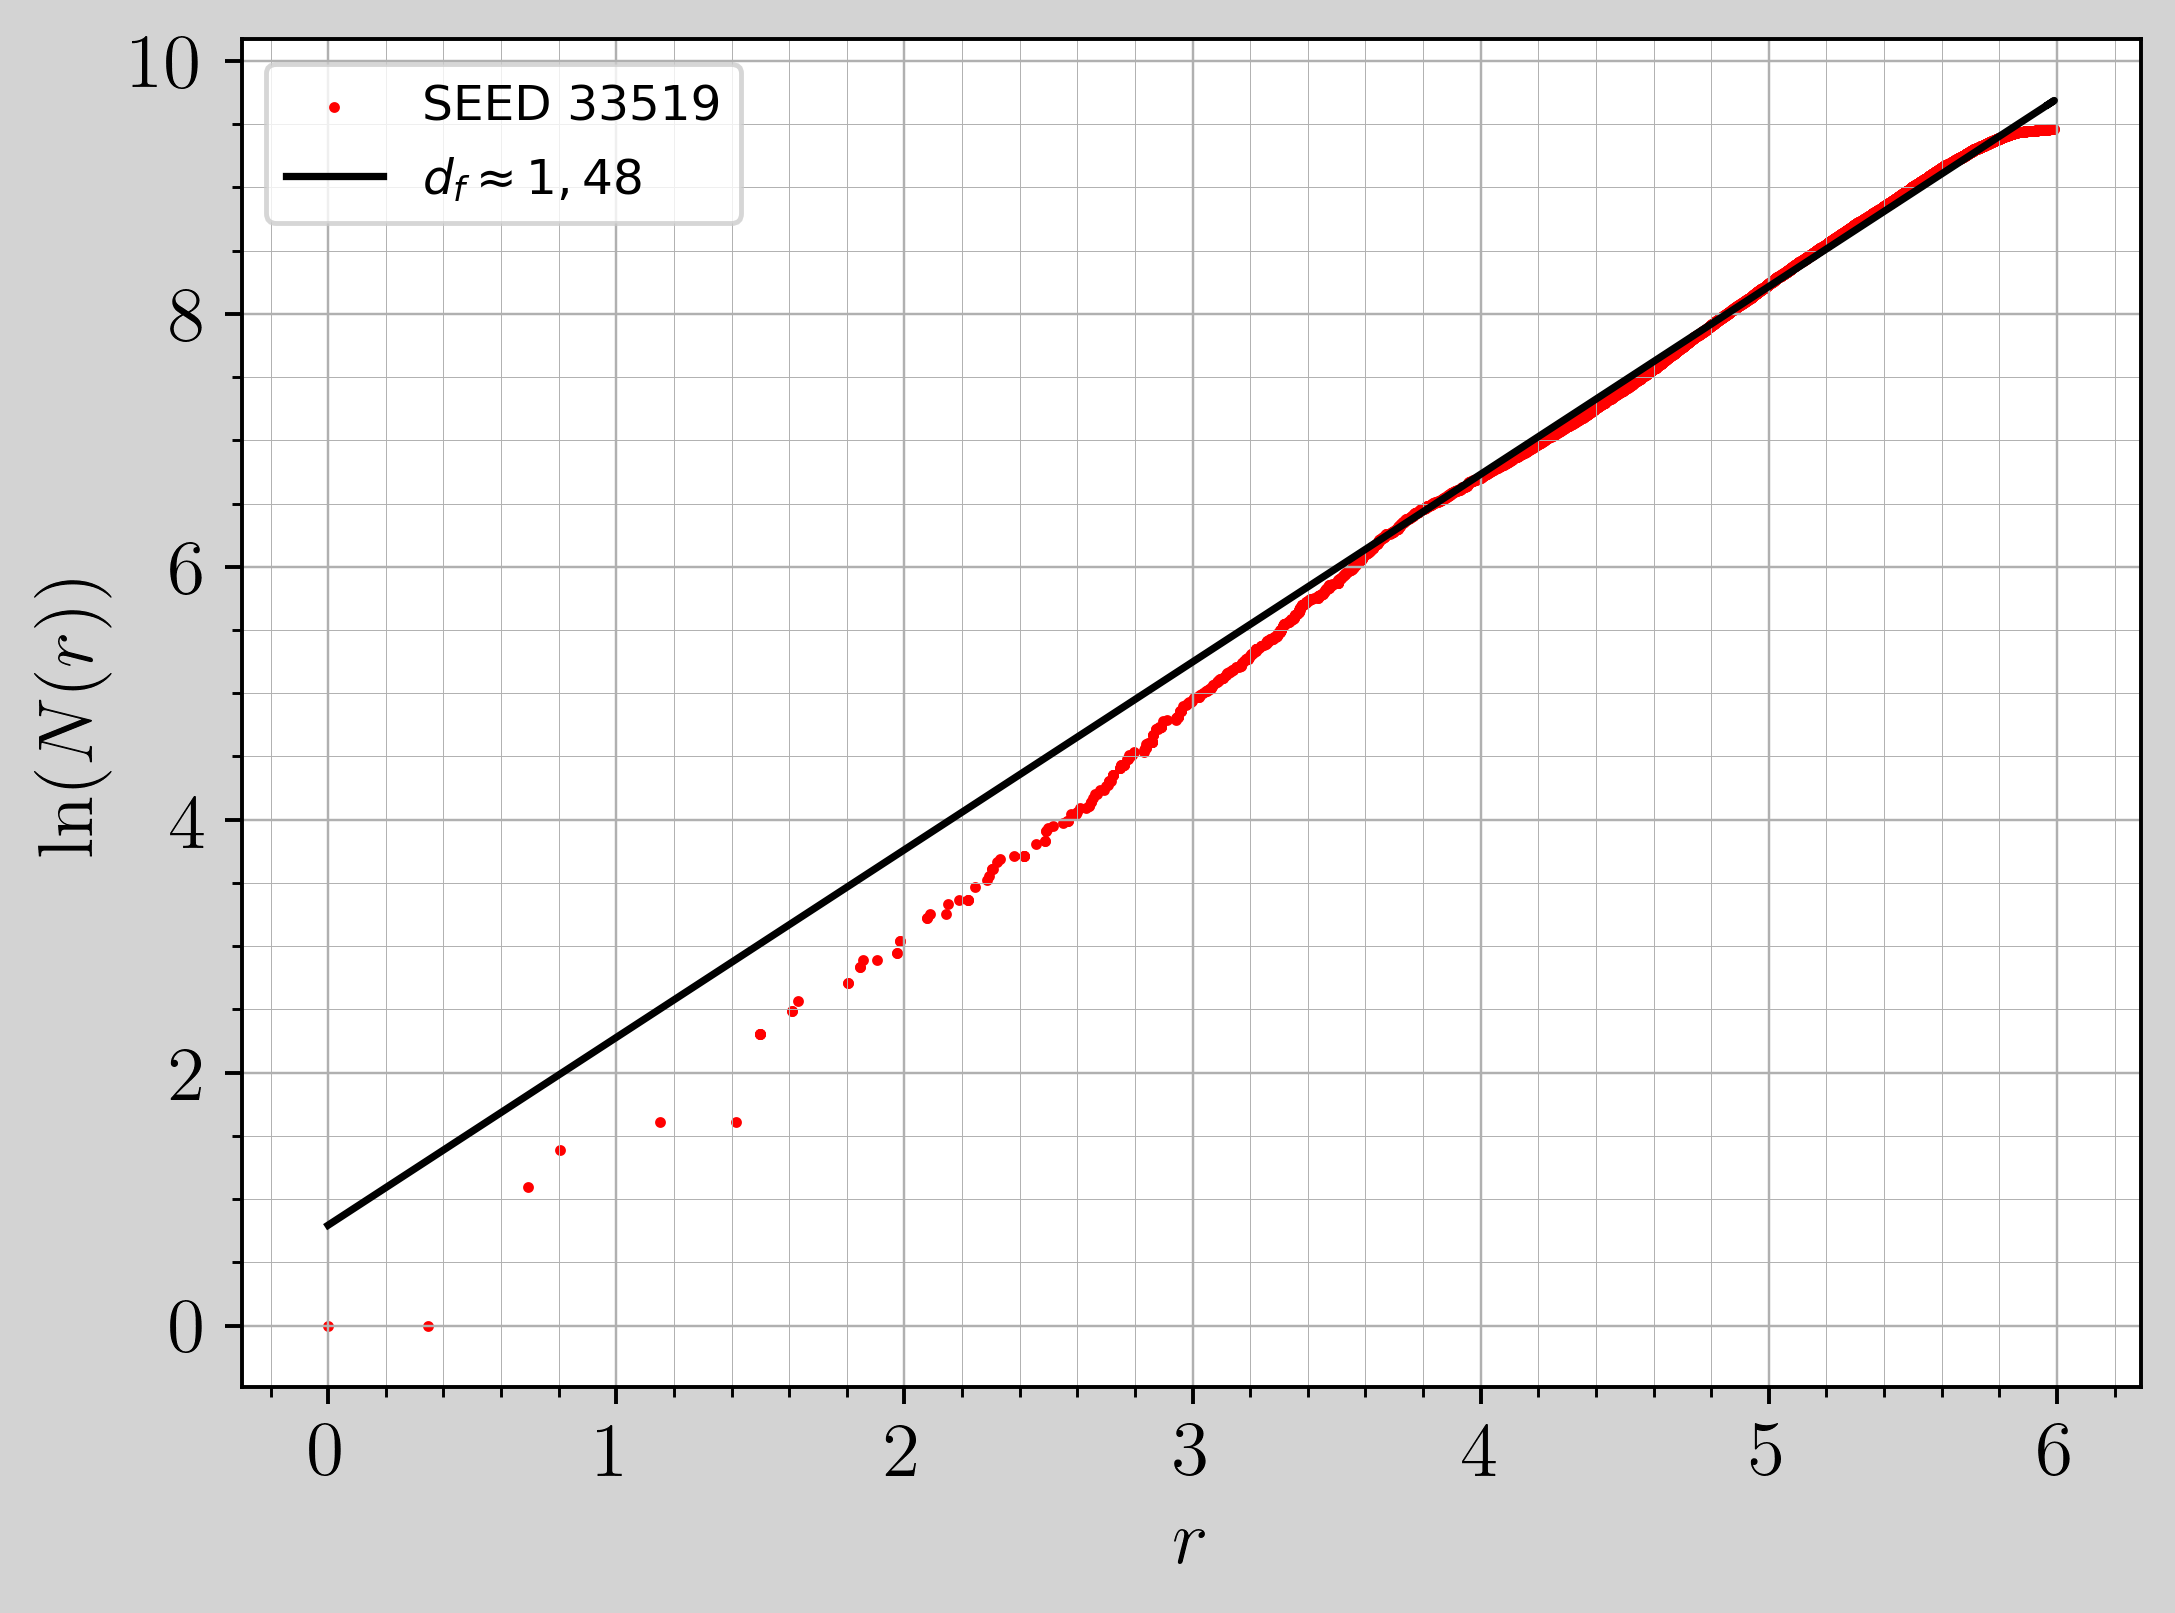
\includegraphics[width=0.7\textwidth]{tarefa-5/rev_popular.png}
  \caption{Ajuste linear para $p = 0.1$.}
  \label{fig:rev_popular}
\end{figure*}


Como podemos ver pela (\ref{fig:rev_popular}) o valor encontrado para a dimensão \( d_f \approx 1.5 \)
não condiz com o esperado \( d_f \approx 1.7 \). Isso porque a forma como contei, externamente, no
graficador é menos precisa que a forma que fiz anteriormente, nas tarefas 2 e 3. A minha solução
para o problema ficou bastante instável e realizar não quis adicionar maior complexidade ao código
para realizar a contagem como anteriormente.
\end{document}

%%% Local Variables:
%%% mode: latex
%%% TeX-master: "main.tex"
%%% End:
